%%
%% Template thesis.tex
%%
\documentclass[12pt,oneside,a4paper]{book}
%\usepackage[palatino]{anuthesis}
\usepackage{graphicx}
\usepackage{xcolor}
\usepackage[left=3cm,top=2.5cm,bottom=2.5cm,right=2cm]{geometry}
\usepackage{amsmath}
\usepackage{amssymb}
\usepackage{gensymb}
\usepackage{thesis}
\usepackage{cite,url,citesort}
\usepackage{caption}
\usepackage[lined,boxed]{algorithm2e}
\usepackage{enumerate}
%\usepackage{epstopdf}
%\usepackage{epsfig}
%\usepackage{makeidx}
%\usepackage{acmnew-xref}

%%%%%%%%%%%%%%%%%%%%%%%%%%%%%%%%%%%%%%%%%%%%%%%%%%%%%%%%%%%%%%%%%%%%%%%
%% Preamble
\title{Investigating the feasibility of laser scanners for autonomous
  navigation of hexacopters in forests}
\author{Daniel Axtens}
\date{\today}

\renewcommand{\thepage}{\roman{page}}

%\makeindex
\begin{document}

%%%%%%%%%%%%%%%%%%%%%%%%%%%%%%%%%%%%%%%%%%%%%%%%%%%%%%%%%%%%%%%%%%%%%%%
%% Title page
\pagestyle{empty}
\thispagestyle{empty}

\begin{titlepage}
  \enlargethispage{2cm}
  \begin{center}
    \makeatletter
    \Huge\textbf{\@title} \\[2.9cm]
    %\Huge\textbf{\thesisqualifier} \\[2.5cm]
    \huge\textbf{\@author} \\[10.5cm]
    \makeatother
    \LARGE ENGN4718\\
    Supervisor: Dr Jon Kim\\[2cm]
    2014
  \end{center}
\end{titlepage}


%%%%%%%%%%%%%%%%%%%%%%%%%%%%%%%%%%%%%%%%%%%%%%%%%%%%%%%%%%%%%%%%%%%%%%%
%% Here begin the preliminaries
%\input frontmatter

%%%%%%%%%%%%%%%%%%%%%%%%%%%%%%%%%%%%%%%%%%%%%%%%%%%%%%%%%%%%%%%%%%%%%%%
%% Dedication (optional)
%\cleardoublepage
%\pagestyle{empty}
%\input dedication

%%%%%%%%%%%%%%%%%%%%%%%%%%%%%%%%%%%%%%%%%%%%%%%%%%%%%%%%%%%%%%%%%%%%%%%
%% Acknowledgements (optional!)
%\cleardoublepage
%\pagestyle{empty}
%\input ack

%%%%%%%%%%%%%%%%%%%%%%%%%%%%%%%%%%%%%%%%%%%%%%%%%%%%%%%%%%%%%%%%%%%%%%%
%% Abstract
\cleardoublepage
\pagestyle{headings}
%\input{abstract}
Abstract!
%%%%%%%%%%%%%%%%%%%%%%%%%%%%%%%%%%%%%%%%%%%%%%%%%%%%%%%%%%%%%%%%%%%%%%%
%% Table of contents
\cleardoublepage
\pagestyle{headings}
\markboth{Contents}{Contents}
\tableofcontents

%%%%%%%%%%%%%%%%%%%%%%%%%%%%%%%%%%%%%%%%%%%%%%%%%%%%%%%%%%%%%%%%%%%%%%
%% Here begins the main text
\mainmatter

\chapter{Aims and Contribution}
\label{cha:aims}

Reproducible research statement!

\chapter{Introduction}
\label{cha:intro}

\chapter{Literature Survey}
\label{cha:litsurvey}

\chapter{Background}
\label{cha:background}

Note \todo{somewhere, not necessarily here} that PSM is subject to
drift and needs to be compensated for.

\chapter{Construction}
\label{cha:construction}

\section{Hardware}
\label{sec:hardware}

\subsection{Laser Scanner and Gimbal}
\label{sec:laser-scanner-gimbal}

The hardware was built in two phases - Mk I around a Hokuyo
UBG-04LX-F01 scanner \cite{scanner1}, and Mk II around a Hokuyo UTM-30LX scanner \cite{scanner2}. 

\subsubsection{Mk I}
\label{sec:mk-i}

Initially, the assembly was built around a UBG-04LX-F01 laser
scanner.

The UBG-04LX-F01:
\begin{itemize}
\item Has a $240\degree$ scanning range.
\item Produces scans of 682 points, each separated by $0.36\degree$.
\item Has a maximum range of 4000mm.
\item Draws 12V.
\item Provides both serial and USB output.
\item Produces 40 complete scans per second.
\end{itemize}

The scanner was fit into a X-CAM X140B gimbal set \cite{gimbal}. 

The X140B:
\begin{itemize}
\item Is a 2-axis brushless gimbal.
\item Is designed to fit Sony NEX5 series cameras.
\item Draws 12V.
\end{itemize}

After removing one of the supports designed for the Sony NEX5 cameras,
the scanner fit neatly into the gimbal and was secured on a temporary
basis with velcro and foam.

However, as the scanner provides only a USB socket, rather than a USB
cable, it had to be positioned so as to provide access to the USB port
through a hole in the top panel of the gimbal. This necessitated
placing the scanner on one side of the gimbal, and quite far forward,
as shown in Figure~\ref{fig:mk1-mount}. To counterbalance this, a
U-bolt was placed on the other side of the gimbal and loaded with nuts
to roughly balance the platform.

\begin{figure}[h!]
  \centering
  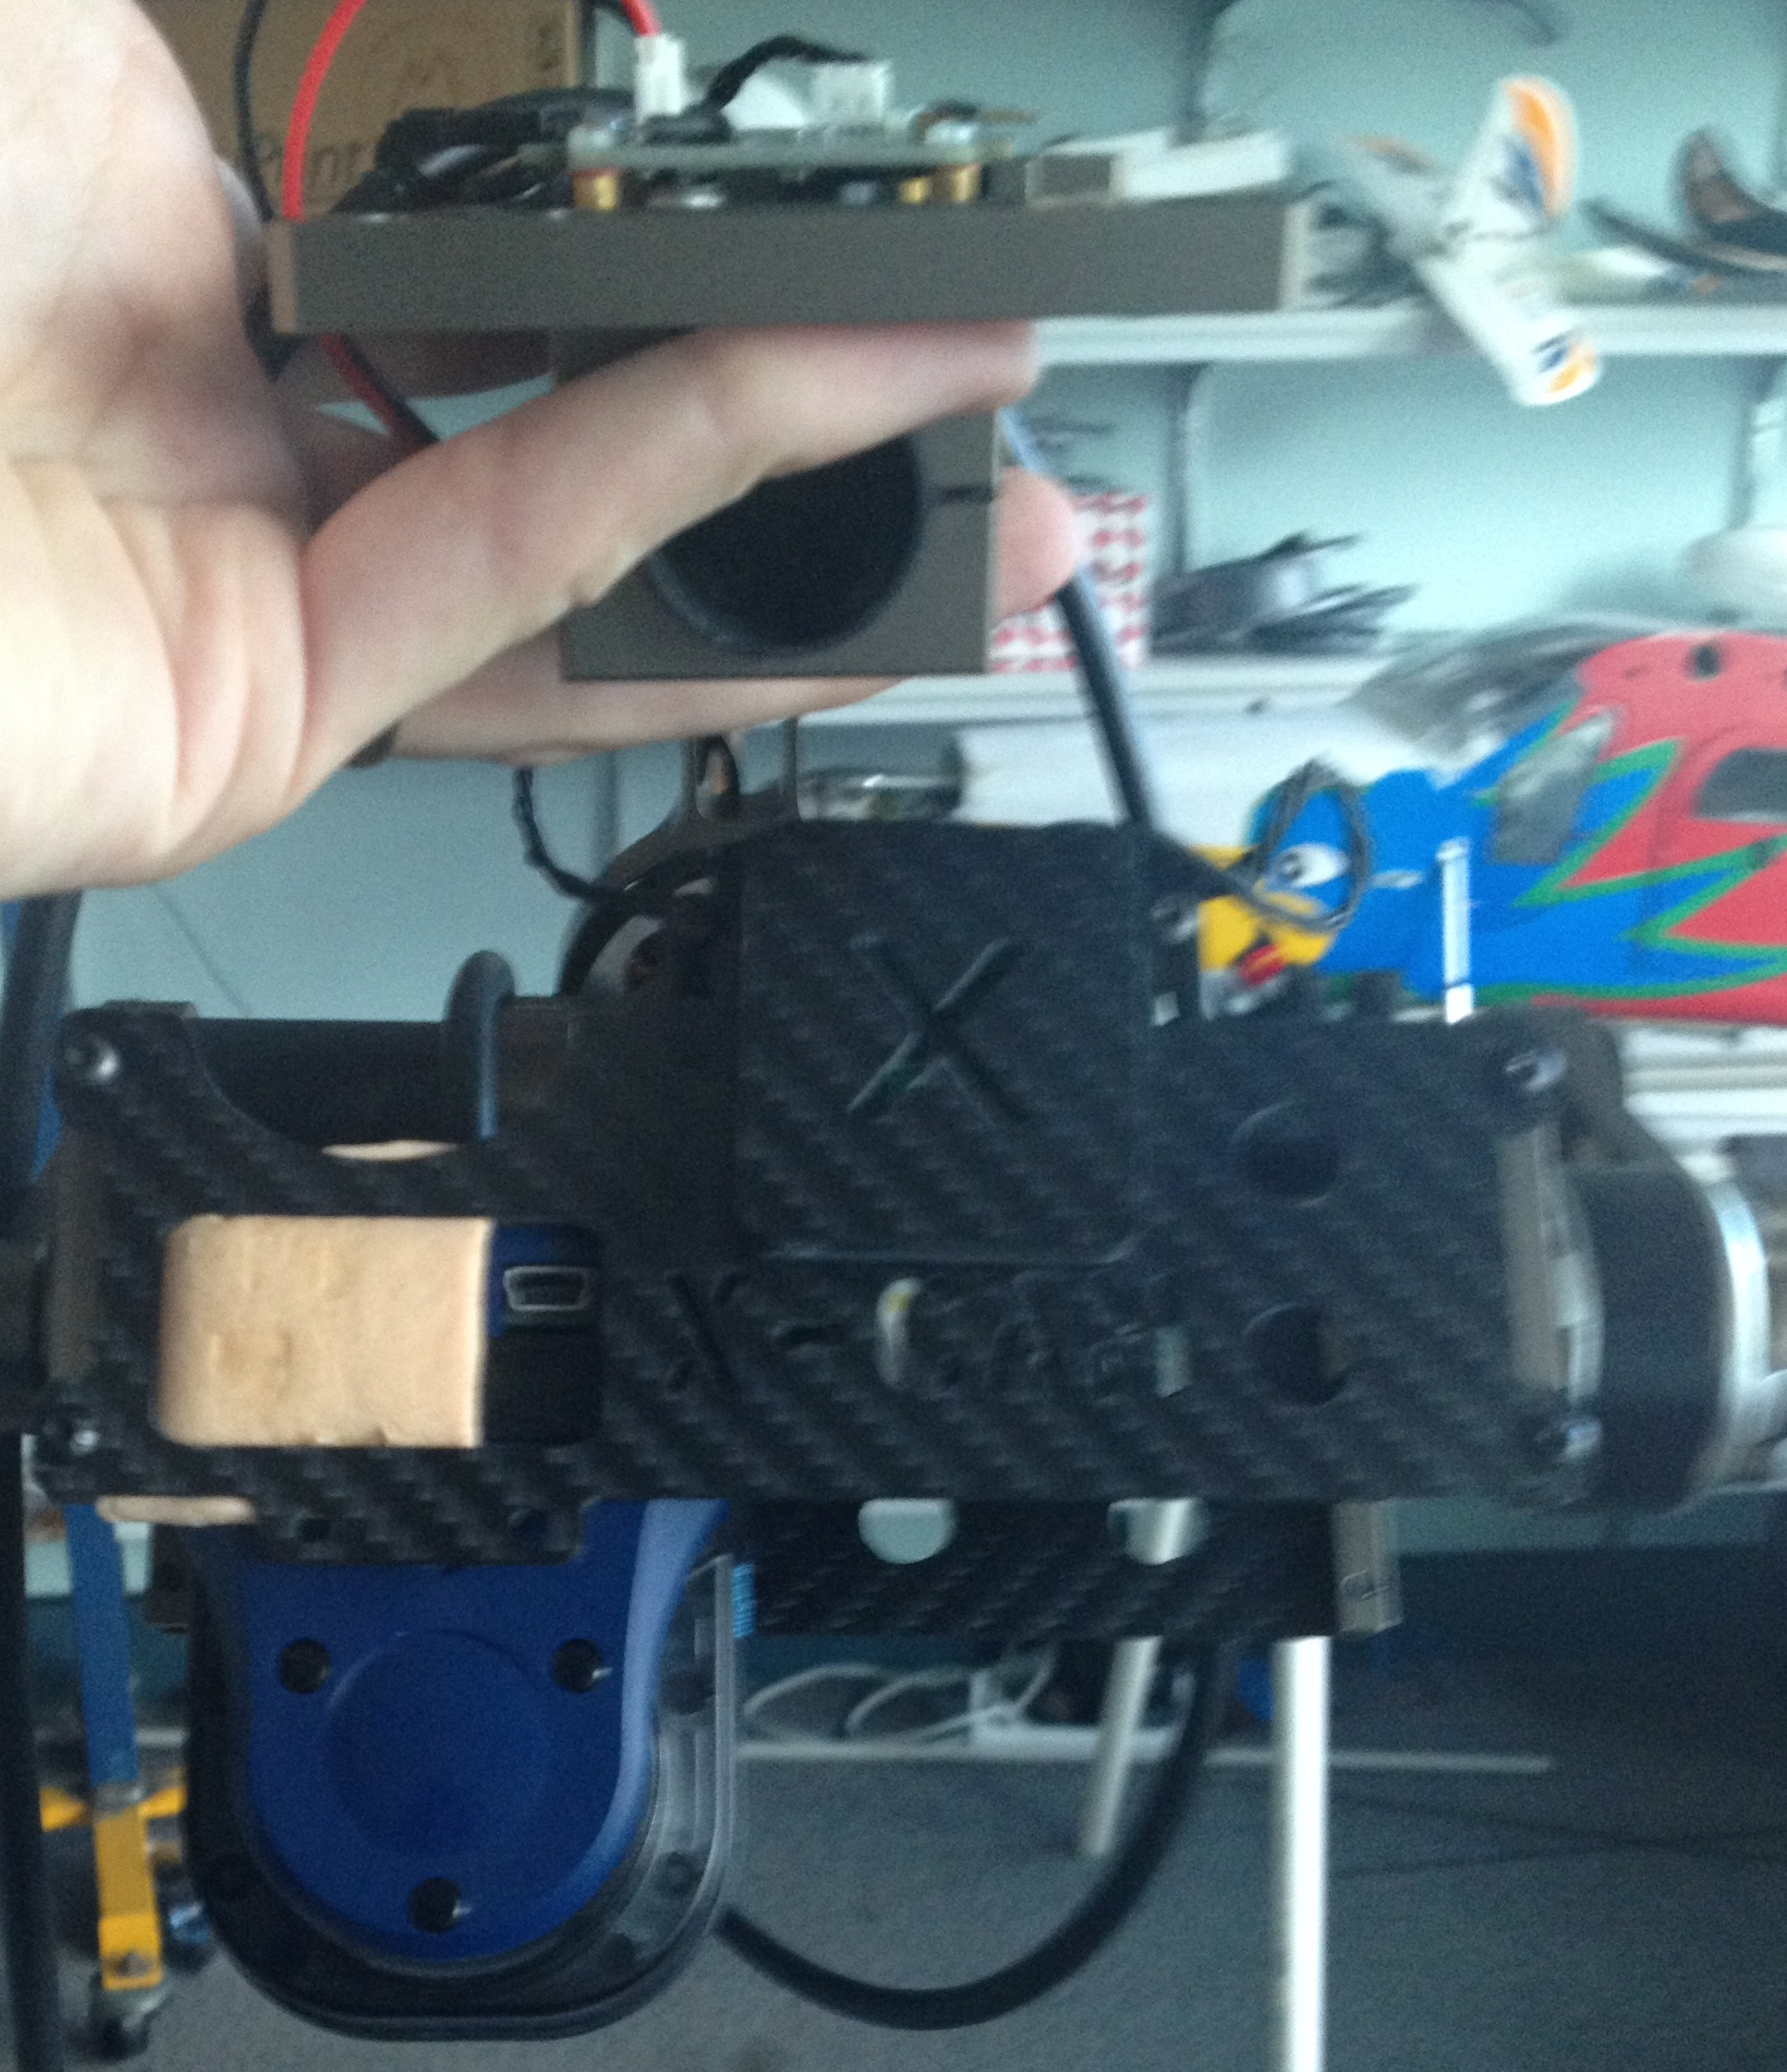
\includegraphics[width=0.5\textwidth]{figs/mk1-mount}
  \caption{Picture of the Mk I, showing the laser scanner mounted with the USB port accessible. This is before the installation of the U-bolt.}
  \label{fig:mk1-mount}
\end{figure}

While this was sufficient to allow testing of the software and mount,
it was excessively heavy and degraded gimbal performance. Designing a
replacement platform was identified as a priority for later stages of the project.

\subsubsection{Mk I Mod II}
\label{sec:mk-ib}

During development, power was accidentally connected backwards across
the gimbal, blowing an IC on the control board. Unhelpfully, the
identifying marks on the ICs were ground off before the gimbal was
shipped, so it was impossible to replace the damaged IC. Instead, the
entire gimbal control system had to be replaced.

The gimbal control board was replaced with a Martinez V3. (See \todo{original site} and e.g. \cite{martinez}.)

The mounting holes in the new board did not fit the existing
mounts for the old board, requiring an adaptor board. \todo{Include
  diagram of adaptor board.}

Replacing the board also necessitated removing the IMU supplied with
the gimbal originally and installing a new one. The new IMU
fortunately fit in the space taken up by the old gimbal, and was
hot-glued in place.

Unlike the old board, this board does not come pre-programmed. The
board runs an Arduino, and the controller software is open-source and
available online \cite{gimbalsoftware}. The software was installed and
tuned. It performed poorly with the heavy Mk I arrangement, but fixing
this was postponed due to the upcoming Mk II.

\subsubsection{Mk II}
\label{sec:mk-ii}

As discussed \todo{somewhere}, it was decided to replace the laser
scanner to improve range and resolution and thus hopefully improver performance outdoors.

The replacement laser scanner was a Hokuyo UTM-30LX scanner
\cite{scanner2}. 

The UTM-30LX:
\begin{itemize}
\item Has a $270\degree$ scanning range.
\item Produces scans of 1080 points, each separated by $0.25\degree$.
\item Has a maximum range of 30m.
\item Draws 12V, between 0.7A and 1A.
\item Provides both serial and USB output.
\item Produces 1 scan every 25ms (40 scans per second).
\item \todo{INTEGRATE THIS!!!} Minimum detectable width at 10m: 130mm.
\end{itemize}

However, this scanner is too tall to fit neatly into the gimbal
mount. As such, a new gimbal base plate was designed in SolidWorks.

\todo{Insert illustration of the gimbal board.}

Only one base plate was fabricated, being laser cut out of 3mm
MDF. After fabrication, the following mistakes were discovered, which
should be corrected should another base plate be fabricated in future:
\begin{itemize}
\item The holes for mounting the rest of the gimbal were designed as
  M2, where as in fact they are M3. (The holes were manually enlarged
  for the sake of expediency.) Version 2 of the board should enlarge
  the holes before laser cutting.
\item Enlarging the holes also requires extending the board so that
  there's enough material on either side of the hole to support the
  weight. (The present board is cutting it perilously close.)
\end{itemize}

The following optimisations could also be made:
\begin{itemize}
\item The existing board has two cut-outs on either side of the
  scanner that were put there for the height sensor. These are
  unnecessary, and should be replaced with a more comprehensive
  weight-reduction strategy.
\item The board is designed with 3 sets of holes, because it was
  unclear where the laser scanner would need to be placed to balance
  the gimbal. As it turns out, it is more balanced than expected, and
  so only the middle set of holes are required. This will allow the
  board to be simplified and reduced in size.
\end{itemize}

The base plate model is available online for future work at
\todo{project url}.

Having fabricated the base plate, the gimbal was
re-adjusted. Performance was \emph{considerably} better than with the
Mk I.

The gimbal controller was initially mounted on nylon spacers above the adaptor board
shown \todo{below}. This was initially laser cut out of 3mm MDF,
however this proved too thick: the original mounting screws were too
short to go through the board and in to the mounts below. A 2mm thick board
proved much more successful.

\subsection{Onboard computer}
\label{sec:onboard-computer}

A Pico-ITX form-factor single-board computer was installed to process
the data in real time. 

The board is a LP-170C \cite{pc}:
\begin{itemize}
\item 1.8GHz Atom processor
\item 4GB memory
\item 4xUSB2 port
\item Compact Flash card for main storage (32GB\todo{check} installed)
\item Draws 12V.
\end{itemize}

The operating system and software set up on the computer is detailed
in the Software section below. \todo{proper reference}

\subsection{Power supply}
\label{sec:power-supply-cons}

The three powered components (gimbal, scanner and PC) all require 12V
power. However, the hexacopter uses 4 cell LiPo batteries, which
provide 14.8V. As such, a buck converter is used to down-convert the
voltage. The convert is shown in
Figure~\ref{fig:converter} below.

\begin{figure}[h!]
  \centering
  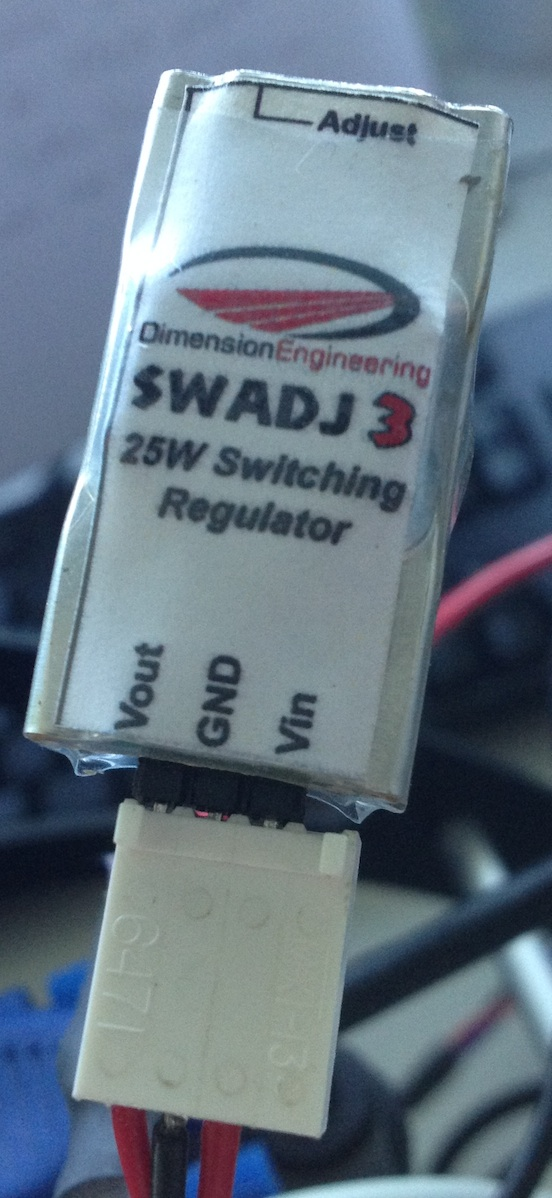
\includegraphics[width=0.33\textwidth]{figs/converter}
  \caption{One of the switching converters}
  \label{fig:converter}
\end{figure}

The converters are rated at 25W. At 12V, this is $\approx 2$A. As
such, it was necessary to split the loads between two converters. One
converter powers the PC and the scanner, and the other powers the
gimbal. A block diagram is shown in Figure~\ref{fig:power} (the
battery, regulator and load all share a common ground).

\begin{figure}[h!]
  \centering
  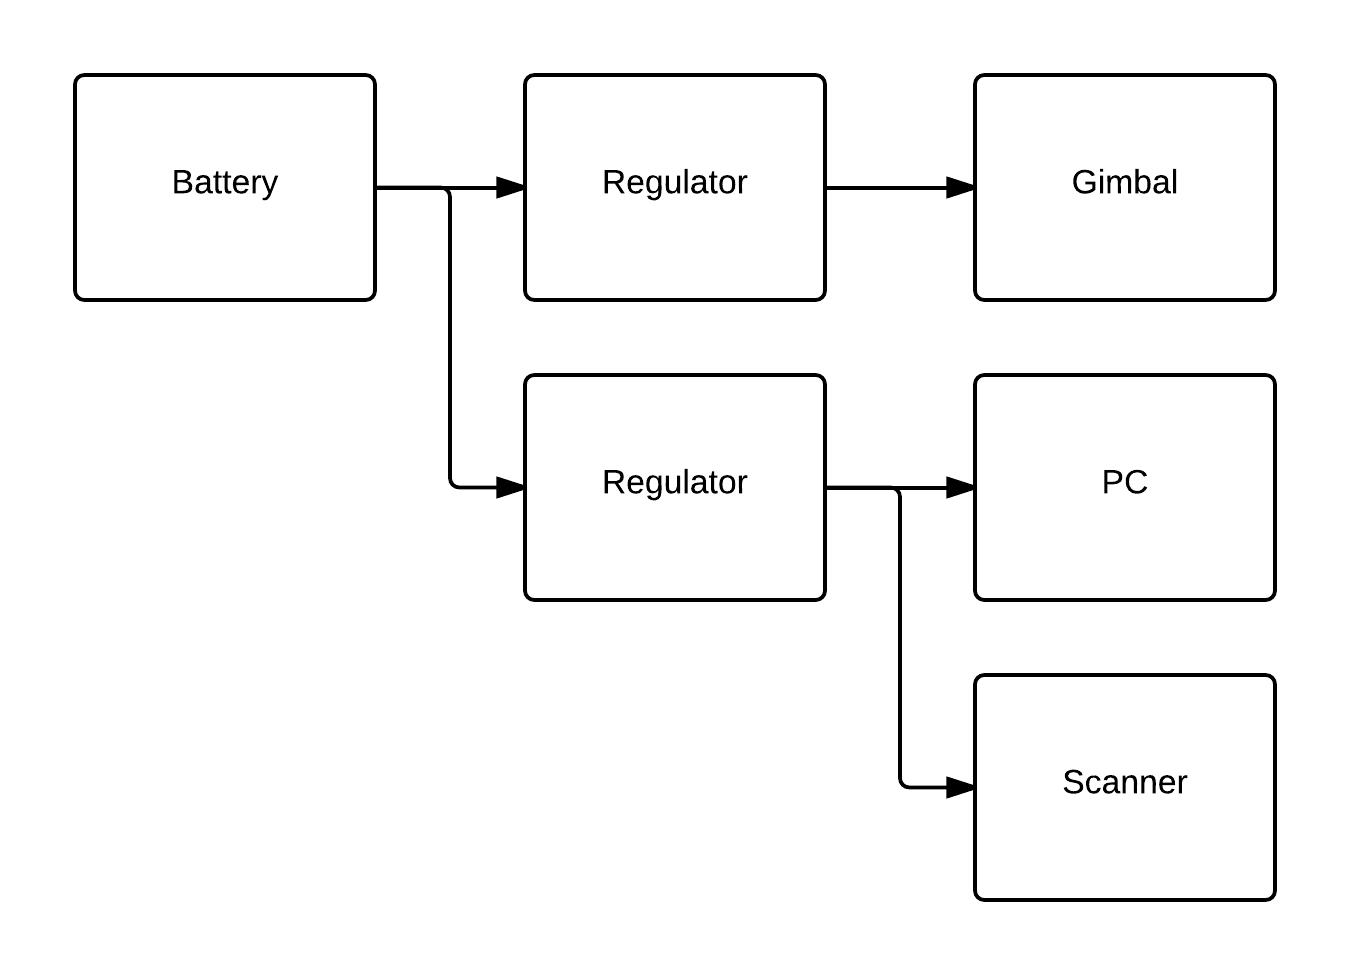
\includegraphics[width=0.5\textwidth]{figs/power}
  \caption{Block diagram of the power system}
  \label{fig:power}
\end{figure}

In addition, a locking connector was installed onto the gimbal
controller board instead of the original two pin connector. (In
addition, the connector can only be inserted one way, eliminating the
chance of destroying another board.)

\subsection{Height measurement setup}
\label{sec:height-meas-setup}

It is desirable for the laser scanner to also be able to provide
information on the altitude of the hexacopter. To this end, a
downwards facing mirror is required, to reflect the last few degrees
of the scan down.

It was desirable for the mirror assembly to be adjustable after
fabrication. As such it was designed so the mirror was held in by two
circular rings, which could be rotated through a mount.

The completed mirror assembly is shown below in
Figure~\ref{fig:mirror}, and the designs in \todo{Figure}.

\begin{figure}[h!]
  \centering
  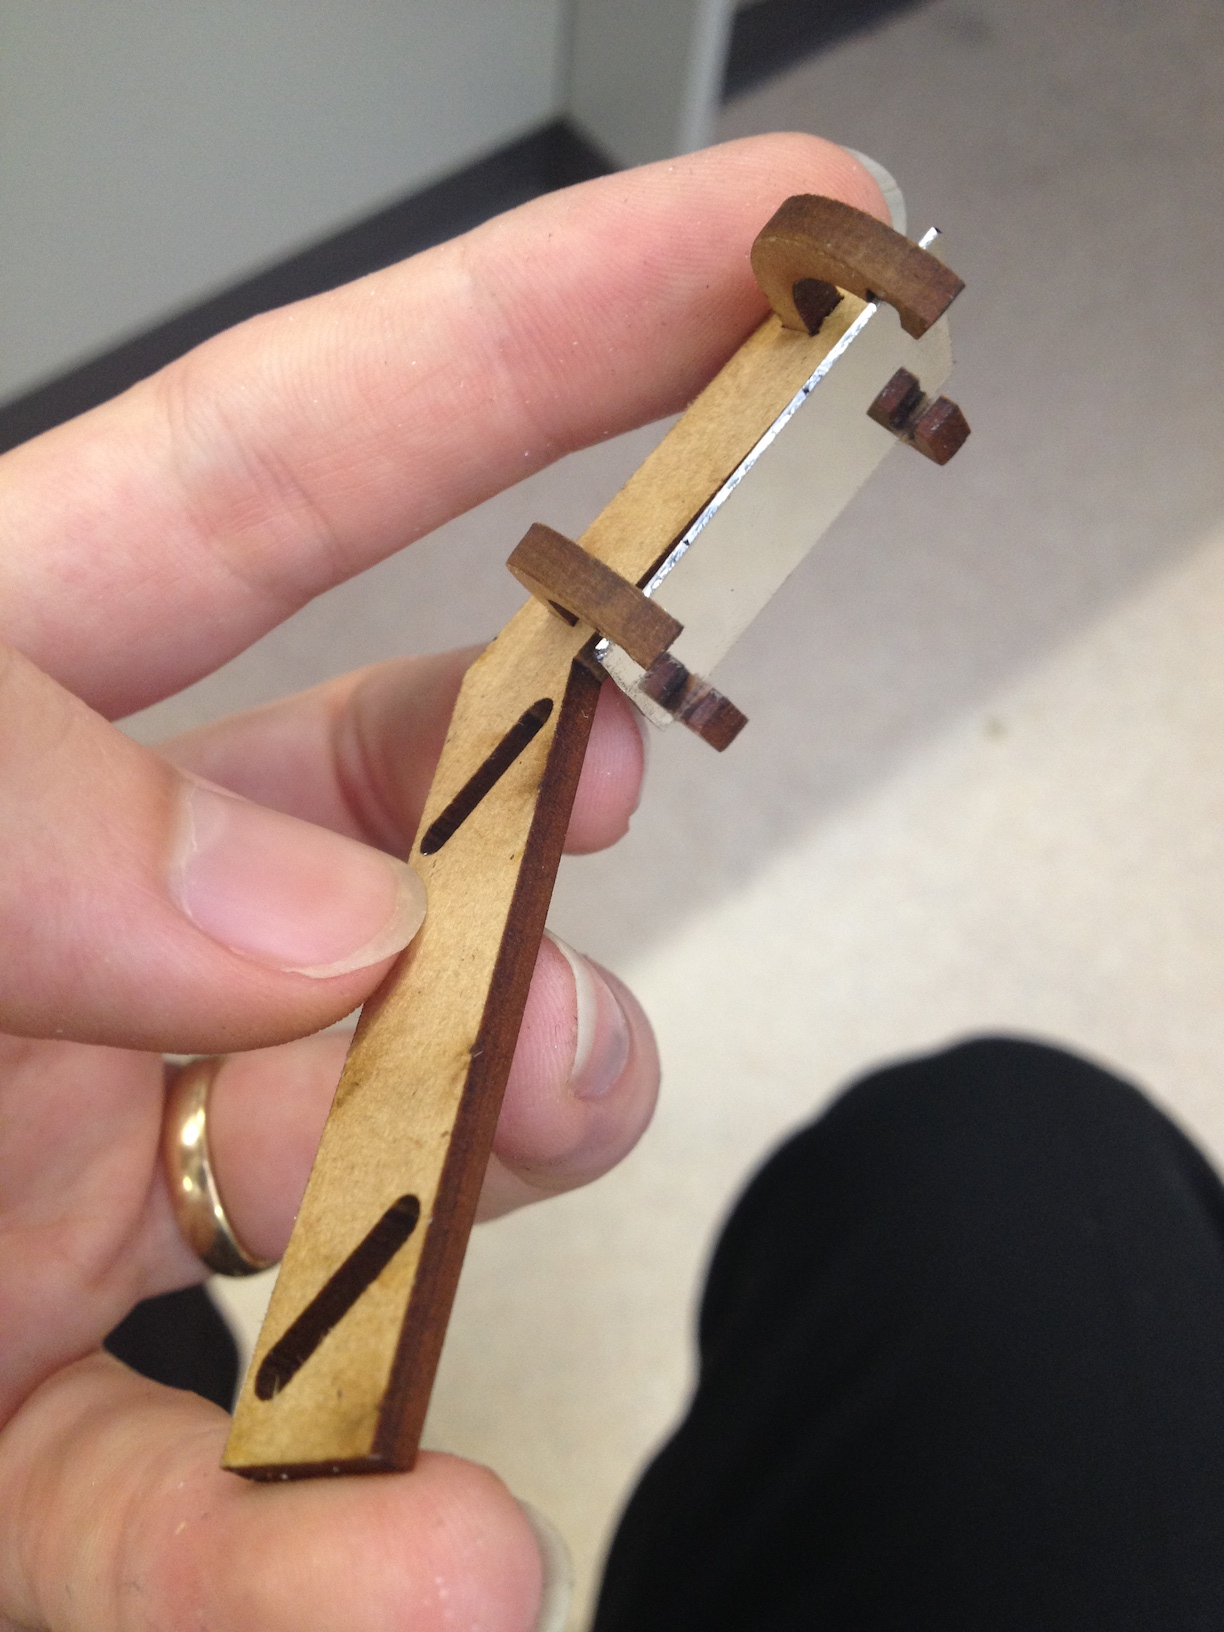
\includegraphics[width=0.45\textwidth]{figs/mirror}
  \caption{The completed mirror assembly (left), \todo{and as installed (right)}.}
  \label{fig:mirror}
\end{figure}

The mirror is a front-faced mirror---silver deposited on silicon---in
order to prevent error from refraction caused by having glass in front
of the reflective surface..

When the mirror was installed, it was discovered that it was too high,
and the entire assembly had to be tilted down and held in place with
hot glue. This assembly mounts on the top of the support - future
assemblies should mount on the bottom side of the top of the support,
with screws going upwards into the support, rather than downwards.

\subsection{Attaching to hexacopter landing gear}
\label{sec:attach-hexac-land}

The gimbal was mounted to an anti-vibration mount with cable
ties. The gimbal control board --- which would otherwise have
protruded too high and hit the mount --- was mounted inside the
anti-vibration mount on velcro. Various adjustments were made to
ensure it does not hit the upper plate of the anti-vibration mount.

The anti vibration mount is attached to a laser cut board designed to
fit the landing gear and the onboard computer. The anti-vibration
mount is attached with cable ties to bear the load and hot glue to
prevent the parts moving with respect to each other.

\todo{The board is reproduced below, along with a model of the
  anti-vibration mount, showing how they mate.}

The board is mounted to the landing gear with cable ties and \todo{hot glue?}.

Figure~\ref{fig:mk2} is a picture of the complete assembly.

\begin{figure}[h!]
  \centering
  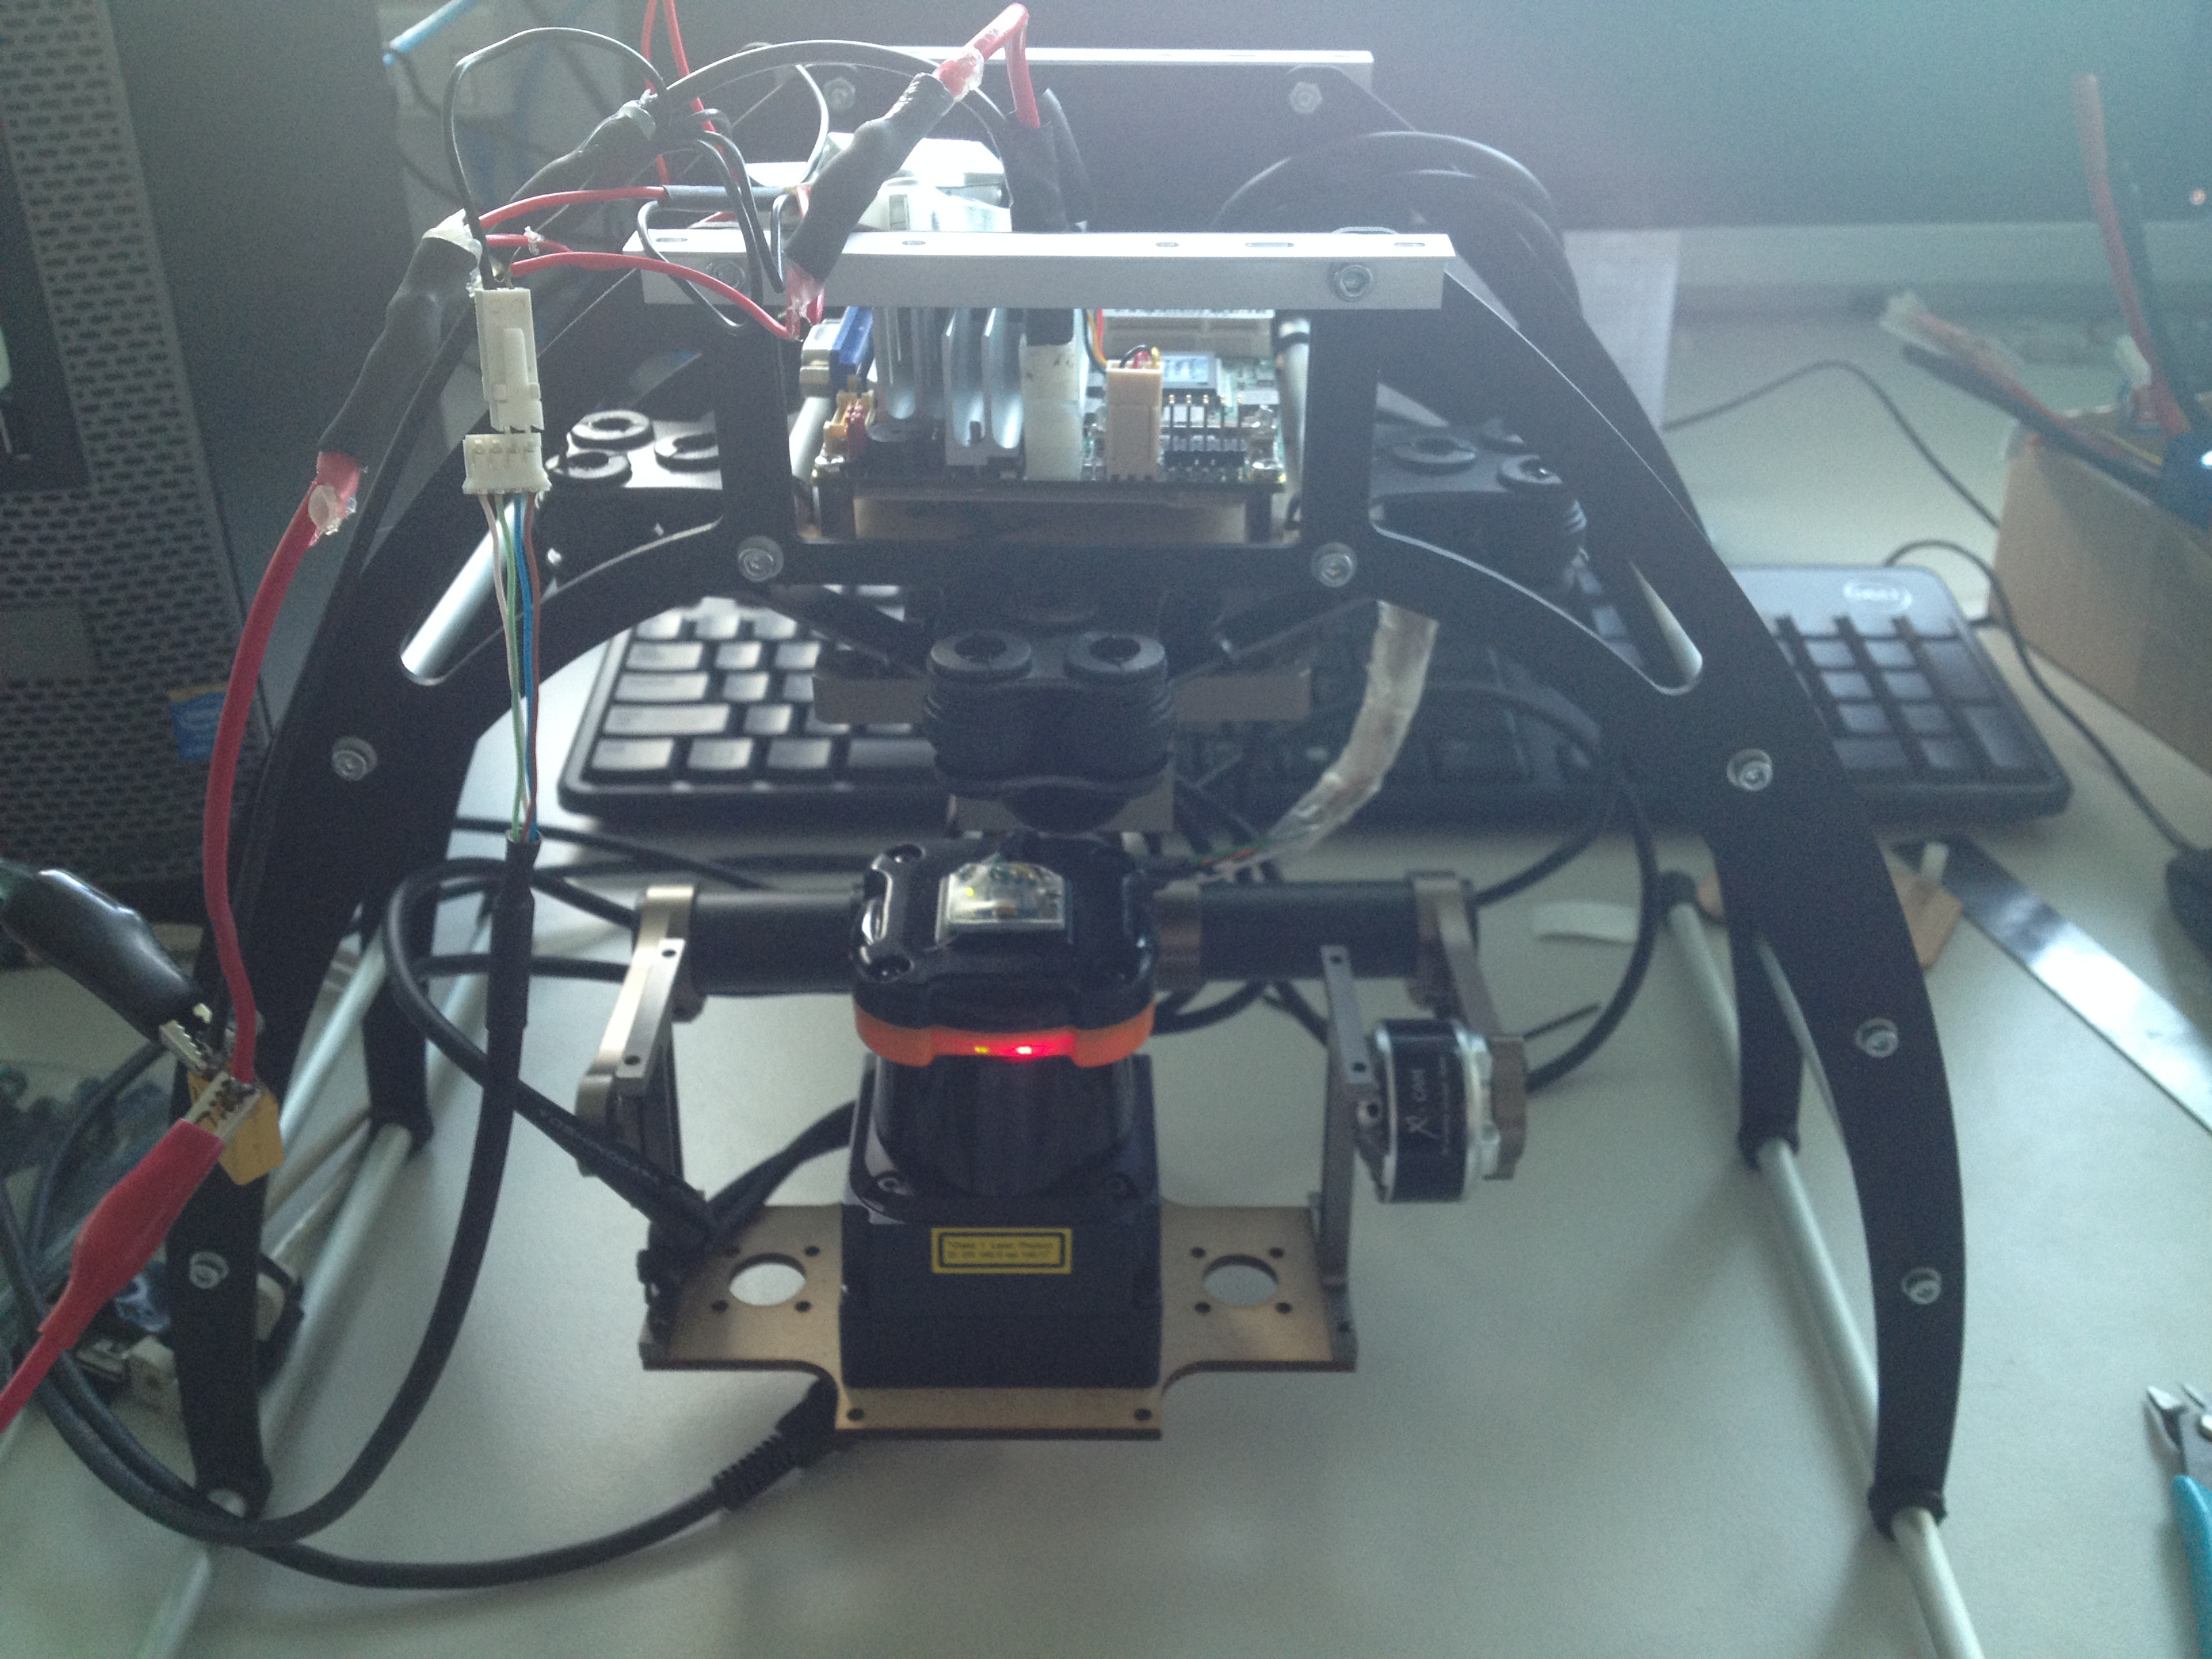
\includegraphics[width=\textwidth]{figs/mk2}
  \caption{The completed assembly. \todo{better image!!!}}
  \label{fig:mk2}
\end{figure}

\section{Software}
\label{sec:software}

The software is built on ROS, the Robot Operating System
\cite{rosos}, using the Indigo version. ROS is built around the
concept of \emph{nodes} --- lightweight, reusable programs that perform a small
part of robot operation --- that are coupled together by passing
around \emph{messages} through use of a publish-subscribe mechanism.

ROS also provides a \emph{transform} mechanism. Loosely, a transform
gives the position of one frame of reference in terms of another frame
of reference. For example, a transform could provide the position of a
sensor with respect to robot body --- a `fixed' transform. Another
example would be a transform that gives the position of the robot body with
respect to some reference frame --- a dynamic transform.

Because ROS is such a modular system, it is helpful to consider an
overview of the setup before the parts are discussed in
detail. Figure~\ref{fig:roschain} shows a graphical representation of
ROS nodes used in the program, as well as the main topics and
transforms. Grey nodes were provided by ROS, while white nodes were
either written or significantly modified during the project.

\begin{figure}[h!]
  \centering
  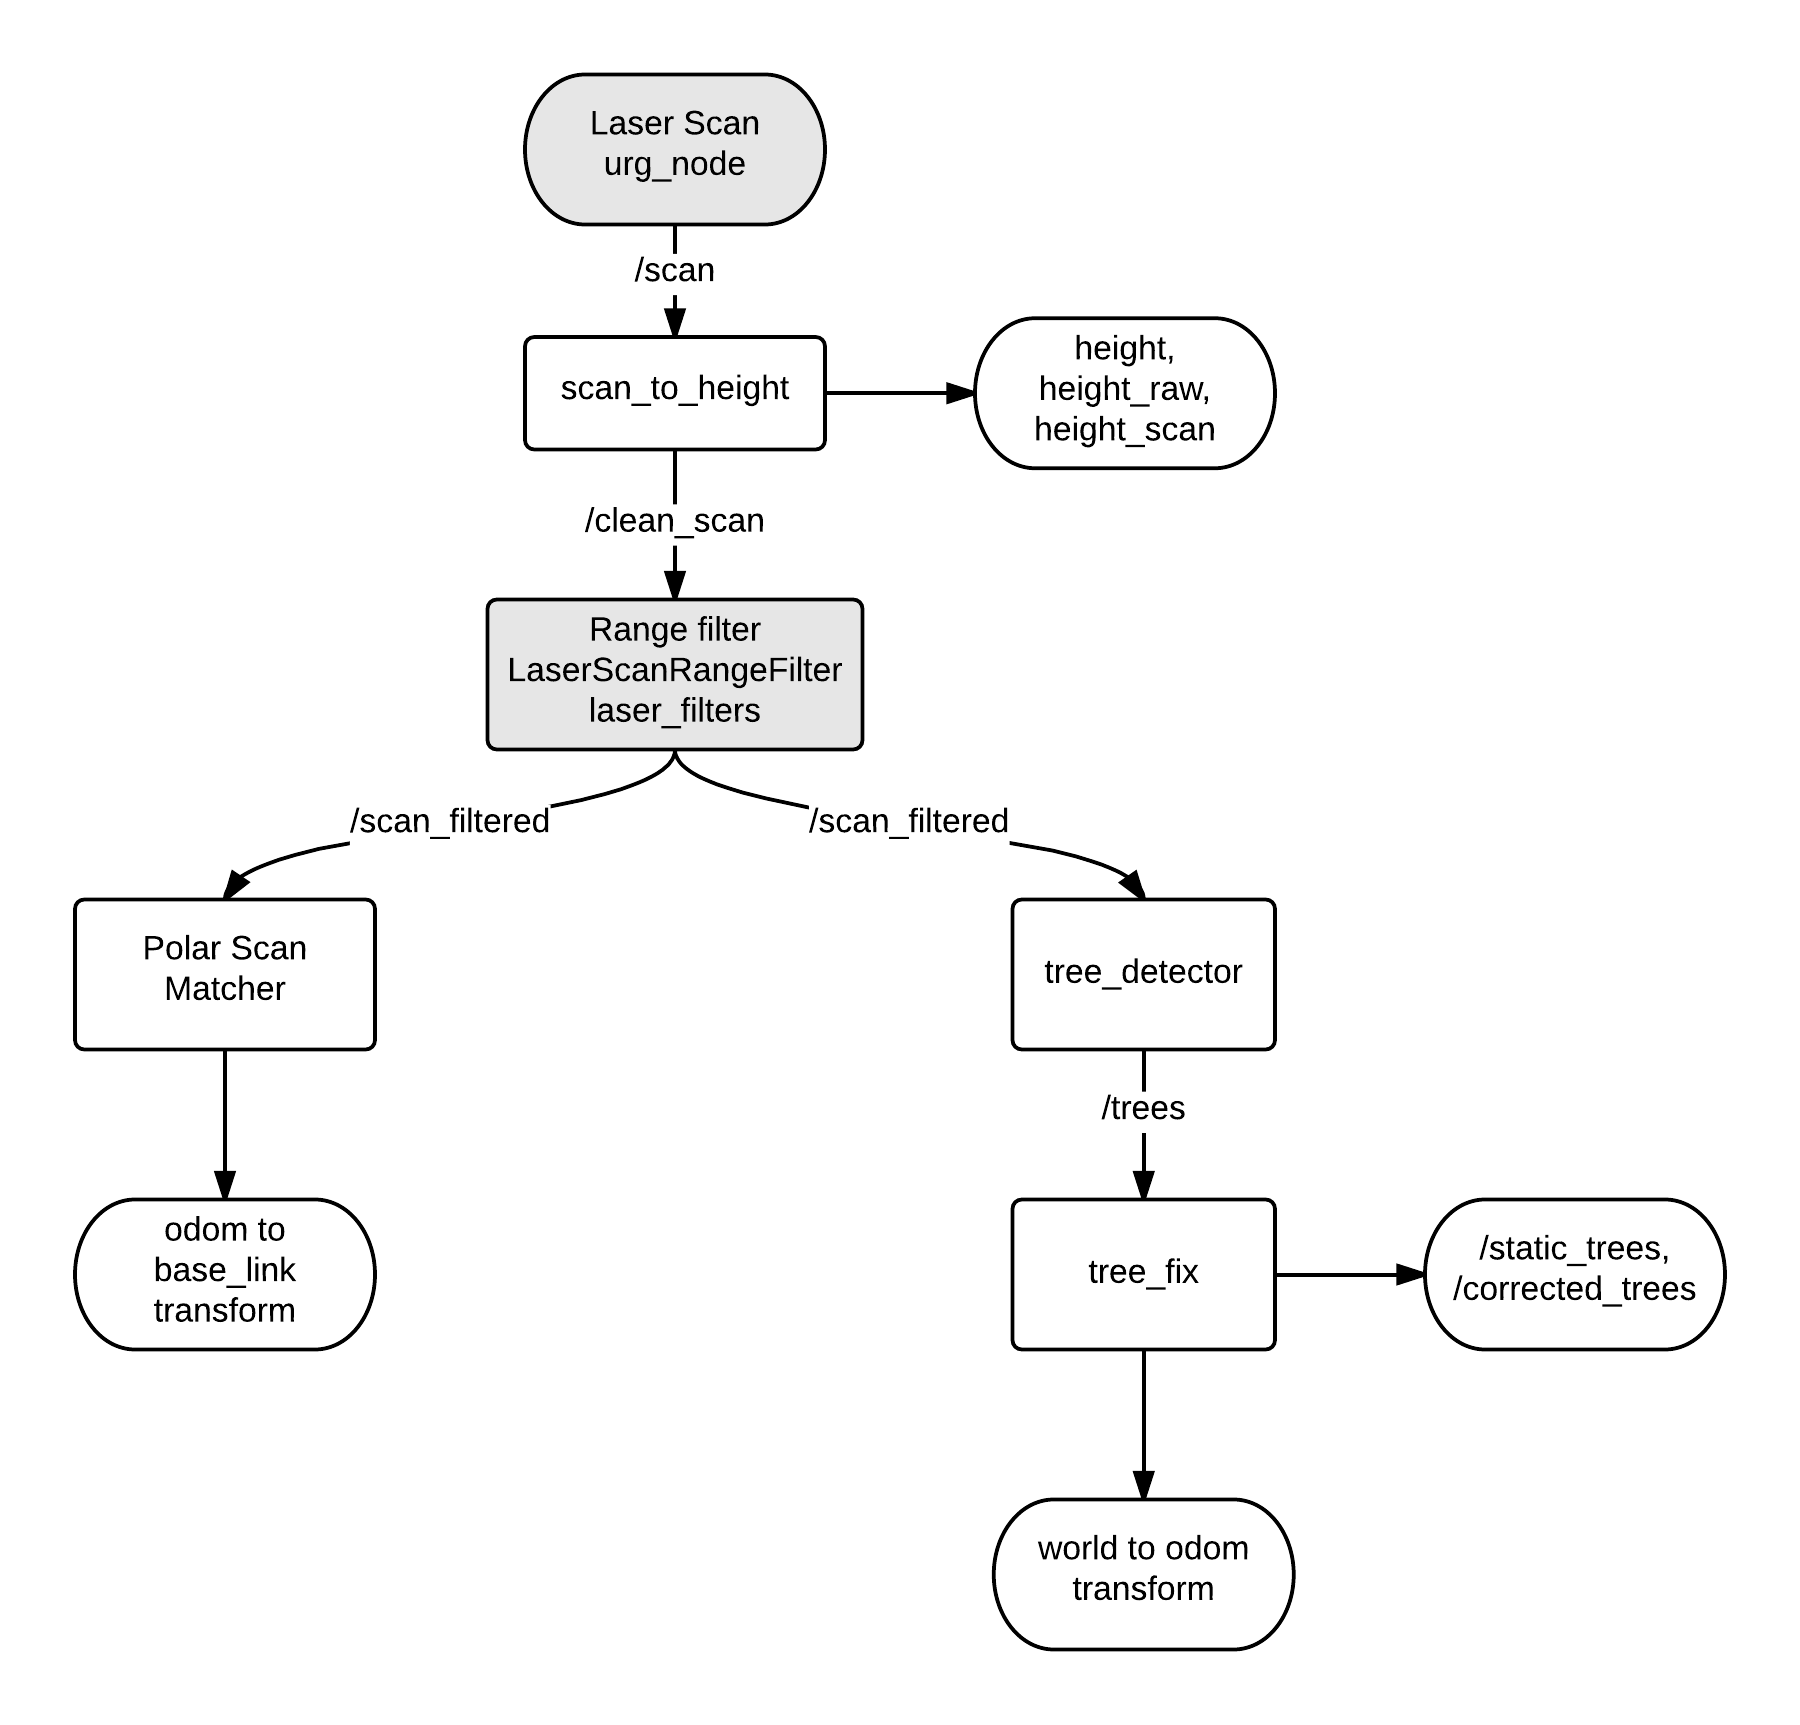
\includegraphics[width=\textwidth]{figs/roschain}
  \caption{Graphical representation of ROS nodes, data passed between
    them, and key transforms published. Grey nodes represent nodes
    provided by ROS. White node were written or significantly modified
  during the project.}
  \label{fig:roschain}
\end{figure}

There are three frames of reference in Figure~\ref{fig:roschain}:
\texttt{world}, \texttt{odom}, and \texttt{base\_link}. They are named
in accordance with ROS standards (\todo{cite REP 105}), and are
defined as follows:
\begin{itemize}
\item \texttt{world} provides a fixed world reference frame. It is
  defined such that the robot starts at the origin.\footnote{For
    complete compliance with REP105, this frame should be name
    \texttt{map}. However, early development wasn't REP105 compliant
    and the name hasn't been updated yet.}
\item \texttt{base\_link} is a frame of reference that is fixed to the
  robot. That is, if there's a sensor attached to the robot, the
  sensor's position remains at a constant position with resepect to
  this frame.
\item \texttt{odom} is difficult to define except in terms of its
  relationship to other frames. The position of \texttt{base\_link} is
  determed by the polar scan matcher with respect to the \texttt{odom}
  frame, and the \texttt{odom} frame is positioned by
  \texttt{tree\_fix} in order to make sure the \texttt{base\_link} frame
  is positioned correctly: that is, the \texttt{world} to
  \texttt{odom} transform is a correction only: \texttt{odom} doesn't
  represent any real position.
\end{itemize}

This is understood most easily through Figure~\ref{fig:rostf}.

\begin{figure}[h!]
  \centering
  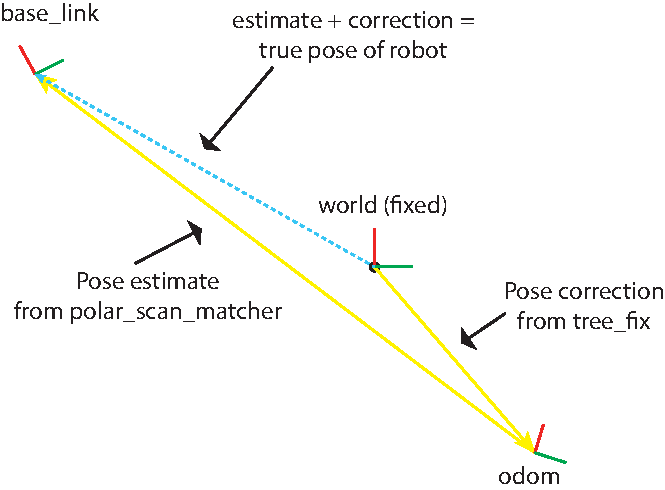
\includegraphics[width=\textwidth]{figs/rostf}
  \caption{A diagramatic explanation of the ROS transforms used.}
  \label{fig:rostf}
\end{figure}

The nodes will now be explained.

\subsection{\texttt{scan\_to\_height}}
\label{sec:scan_to_height}

As explained in Subsection~\ref{sec:height-meas-setup}, the last few
points of the laser scan are reflected downwards to get a measurement
of height.

This node splits the received laser scan (topic \texttt{/scan}) into
two scans: \texttt{/height\_scan}, which contains just the points for
the downward reflected height, and \texttt{/clean\_scan} - the scan
with the downward reflected points removed.

The downward points are then averaged\footnote{\todo{mean or
    median?}}, and this value published in
\texttt{/height\_raw}. However, this value is very noisy. \todo{How noisy?}

To reduce the noise, the value is then included in a \todo{10?}  point moving average, and
that value published in \texttt{/height}. This has a very low noise
--- in the order of a couple of centimetres --- but because there are
40 scans per second, still very rapid response to changes in altitude.

So far, this value is unused. Future work should integrate this into
control of the hexacopter.

\todo{Correction: There are two sources of error in the height
  measurement.} Firstly, the mirror is not at a perfect downwards
angle, so there is a multiplicative error. Secondly, there's an
additive error due to the distance between the sensor and the mirror,
and due to losses caused by the mirror surface. These \todo{will be}
both corrected for.

\subsection{Scan Filtering}
\label{sec:scan-filtering}

Having the laser scanner mounted in the landing gear means that
various points of the scan will always hit the landing gear. If these
are not filtered out, they cause the polar scan matching to perform
very poorly.

A node provided with ROS is used to filter points from the scan that
would be within the footprint of the hexacopter. This significantly
improves performance.

Various other filters were explored, including a shadow remover, and
an interpolation filter. Neither improved performance.

\subsection{Polar Scan Matcher}
\label{sec:polar-scan-matcher}

The polar scan matcher is based on \todo{citation needed - original
  paper for PSM}.

This node posed a number of challenges.

Firstly, while code was purported to exist for ROS, it no longer
existed in the main \texttt{scan\_tools} repository \todo{cite the
  ccny repo}. A copy was located in another repository and copied
over.

Secondly, the code was old - circa ROS Electric, and would not compile on more recent
versions of ROS due to changes in various libraries, specifically the
transform datatypes.\footnote{\todo{ref:}
  \url{http://wiki.ros.org/geometry/bullet_migration},
  \url{http://wiki.ros.org/fuerte/Migration}} Fortunately, the
provided migration scripts proved sufficient to migrate the code and
have it compile.

Thirdly, the code once compiled did not run, but would crash almost
immediately after launching. The code initially expected the scanner
to report a range of 0 for out of range points, but the scanner was
instead reporting NaN (not a number) values instead. Fixing the
assumption lead to the polar scan matcher running reasonably well.

These changes were sufficient to get the laser scanner working
reasonably well indoors, but completely inadequately outside. The
first attempt to fix this was by replacing the scanner with a much
more capable scanner (see the Mk II: Subsection~\ref{sec:mk-ii}). This
lead to some improvement but not enough to make the system usable.

The following changes were also required for acceptable outdoor
performance:

\begin{description}
\item[Negative Distances] Error reports from the polar scan matcher node
  showed that occasionally negative distances were found. Tracing
  these back, it was discovered that the scanner node itself was
  outputting negative distances. These were discarded in an early
  stage of processing, leading to slightly improved performance.
\item[Median Filter] A close examination of the code revealed that one
  of the pre-processing steps was a median filter.

  The median filter replaces each point with the median of the points
  around it. Formally, it works as follows:
  \IncMargin{1em}
  \begin{algorithm}
    \KwIn{Laser scan $s$}
    \KwOut{Laser scan $s'$}
    \BlankLine
    \For{$i \leftarrow 0$ \KwTo $(\text{length of }s - 1)$}{
      \tcp{Collect 5 points: the point and two points either side.}
      $r \leftarrow s[(i-2) \ldots (i+2)]$ \;
      $r' \leftarrow \text{bubble\_sort}(r)$ \;
      \tcp{Replace the point with the central (3rd) point of $r'$}
      $s'[i] \leftarrow r[2]$ \;
    }
    \caption{Psuedo-code for the median filter algorithm}
  \end{algorithm}

  While this algorithm works well indoors, where there are long
  straight runs, the algorithm unfortunately dramatically
  impedes outdoor performance. Disabling this filter entirely lead to
  vastly superior outdoor behaviour.
\end{description}


\subsection{Tree Detection \& Localization}
\label{sec:tree-detection-localization}

\todo{Some form of introduction: reference previous post-processing
  work, explain that this now provides that in real time.}

In keeping with the ROS philosophy of having small, specialised and
reusable nodes, the process is broken up into two nodes: one which
takes laser scans and detects trees, and one which uses the detected
trees to correct the polar scan matching-derived position to a true
position.

\subsubsection{\texttt{tree\_detector}}
\label{sec:tree_detector}

The tree detector node simply detects trees from a laser scan.

It's presently a very primitive process, but works sufficiently well
when the following assumptions are met:
\begin{itemize}
\item Trees are close. More precisely, a \emph{map range} is defined,
  and points that compose the trees must be within the square
  (-\texttt{MAP\_RANGE}, -\texttt{MAP\_RANGE}) to (\texttt{MAP\_RANGE},
  \texttt{MAP\_RANGE}). The choice of \texttt{MAP\_RANGE} is a trade-off
  between detection range and speed and memory usage. However,
  increasing range has diminish returns, as the distance between
  detected points grows with distance, making it harder to accurately
  detect trees. Experimentally, 6 metres \todo{check?} provides good results.
\item There are no other significant clusters of points (e.g. no
  walls) within the map range.
\end{itemize}

The process proceeds as follows:
\begin{description}
\item[Drop scans] Only 1 out of every $N$ scans are processed, where
  $N$ is a parameter currently set to \todo{verify} 8. This is
  necessary to ensure that there's not a backlog of messages out of
  the node. Drop the other $N-1$ scans without processing them.
\item[Convert the laser scan into an image] For speed and memory usage
  reasons, only points within the map range are included. Presently,
  the intensity of the reading from the laser scan is ignored, and
  readings are mapped either to pure white if they fall within the map
  square, and black if they don't fall within the map.
\item[Blur] A gaussian blur is applied to the image. This serves two
  purposes:
  \begin{itemize}
  \item It reduces the effect of noise on future stages - a stray
    reading will be blurred into basically nothing.
  \item A scan of a tree at a few metres distance will not be a
    contiguous line, due to the angle between the readings. This leads
    to it not being detected as one feature, but as several, which is
    undesirable. Blurring tends to create smoother, contiguous runs
    that are easier to detect.
  \end{itemize}
\item[Threshold] A threshold is applied to further reduce noise.
\item[Circle detection] Actually detecting circles was more difficult
  than expected. Four major approaches were attempted:
  \begin{itemize}
  \item The OpenCV built-in ``Hough Circles'' detection process. This
    failed to yield any results at all, even on artificial perfect
    circles and with supplied sample code. This may be due to a bug
    introduced in OpenCV, as in \todo{cite emails were someone else
      had the bug}.
  \item Feature detection with a semi-circle also failed; which is
    apparently due to the same root cause as the Hough Circles
    failure.
  \item MSER---maximal stable external regions---a way to detect
    `blobs', was mostly successful, but far too slow.
  \item The approach ultimately adopted was to find features with more
    points than a given threshold, and find the minimum enclosing
    circle. While not strictly accurate, it provides sufficient
    accuracy, especially when there are a sufficiently large number of
    points, for the algorithm to work well.
  \end{itemize}
\item[Publish points] The centers of the detected trees are published
  as a point cloud to the \texttt{/trees} topic. They're published in
  the same frame of reference that they're detected in ---
  \texttt{/laser}, which in the current implementation is tied to
  \texttt{/base\_link}.
\end{description}

Significant future work is needed to make this node more
robust and versatile, especially in an outdoor environment that
contains both trees and other objects. The biggest improvement needed
is to replace the circle detection algorithm with a proper one, such
as RANSAC \todo{citation}. This will prevent features like walls from
being inadvertently detected as trees.

Furthermore, there are a number of improvements that can be made to
the speed and robustness of the algorithm.
\begin{itemize}
\item Presently, the points are placed into a map, which, for memory
  and speed reasons, is fairly small. However, the map is very sparse,
  because in an outdoor environment most of the points are out of range.
  It should be fairly straightforward to create several smaller maps
  wherever points are detected, decreasing memory usage, increasing
  speed, and increasing detection range.
\item A gaussian filter is used with quite a large kernel ($11 \times
  11$ pixels). Alternative, faster filters should be evaluated.
\item The entire Python code should be re-written in C++, which would
  probably result in a \emph{significant} speed up.
\item The feasibility of processing the entire scan in its original
  polar form should be considered. \todo{what happens when you
    transform a semicircle into polar form? - it appears to become an
    semi-ellipse...}
\end{itemize}

Finally, it would be highly desirable for many of the hardcoded
parameters to be made configurable in the standard ROS way.

\subsubsection{\texttt{tree\_fix}}
\label{sec:tree_fix}

The \texttt{tree\_fix} node uses the trees published by
\texttt{tree\_detector} to perform primitive SLAM. Specifically, \texttt{tree\_fix}:
\begin{itemize}
\item Builds up a map of the trees in the environment.
\item Uses that map and the detected trees to localise the robot,
  providing a correction to the pose estimate provided by the polar
  scan matcher.
\end{itemize}

In very broad brush strokes, the process is as follows:
\begin{itemize}
\item Assume that the change between this scan and the last scan is
  probably not too great, seeing as the \texttt{tree\_fix} package
  publishes a new point cloud on \texttt{/trees} several times a
  second. Therefore, we can use the last correction to gain a good
  first estimate of what the current correction should be.
\item Find the static points closest to the new points, so we have a
  two sets of points of equal length. 
\item Then it becomes the case that:
  \begin{equation}
    \label{eq:1}
    P' = RP + T + N
  \end{equation}
  That is, the new points ($P'$) is the rotation ($R$) of the original
  points ($P$) plus a translation ($T$) plus some noise/error ($N$).

  Therefore, we can determine the $R$ and $T$ that minimises the error
  between the known points and $P'$.
\item We use the $R$ and $T$ to transform the complete set of new
  points. 
\item Points that cannot be matched to existing map points are
  determined to be new trees and added to the map.
\end{itemize}

Implementation details make the algorithm more complex in
practise. The implemented algorithm is shown in
Figure~\ref{fig:tree_fix} and fleshed out in more detail below.

\begin{figure}[h!]
  \centering
  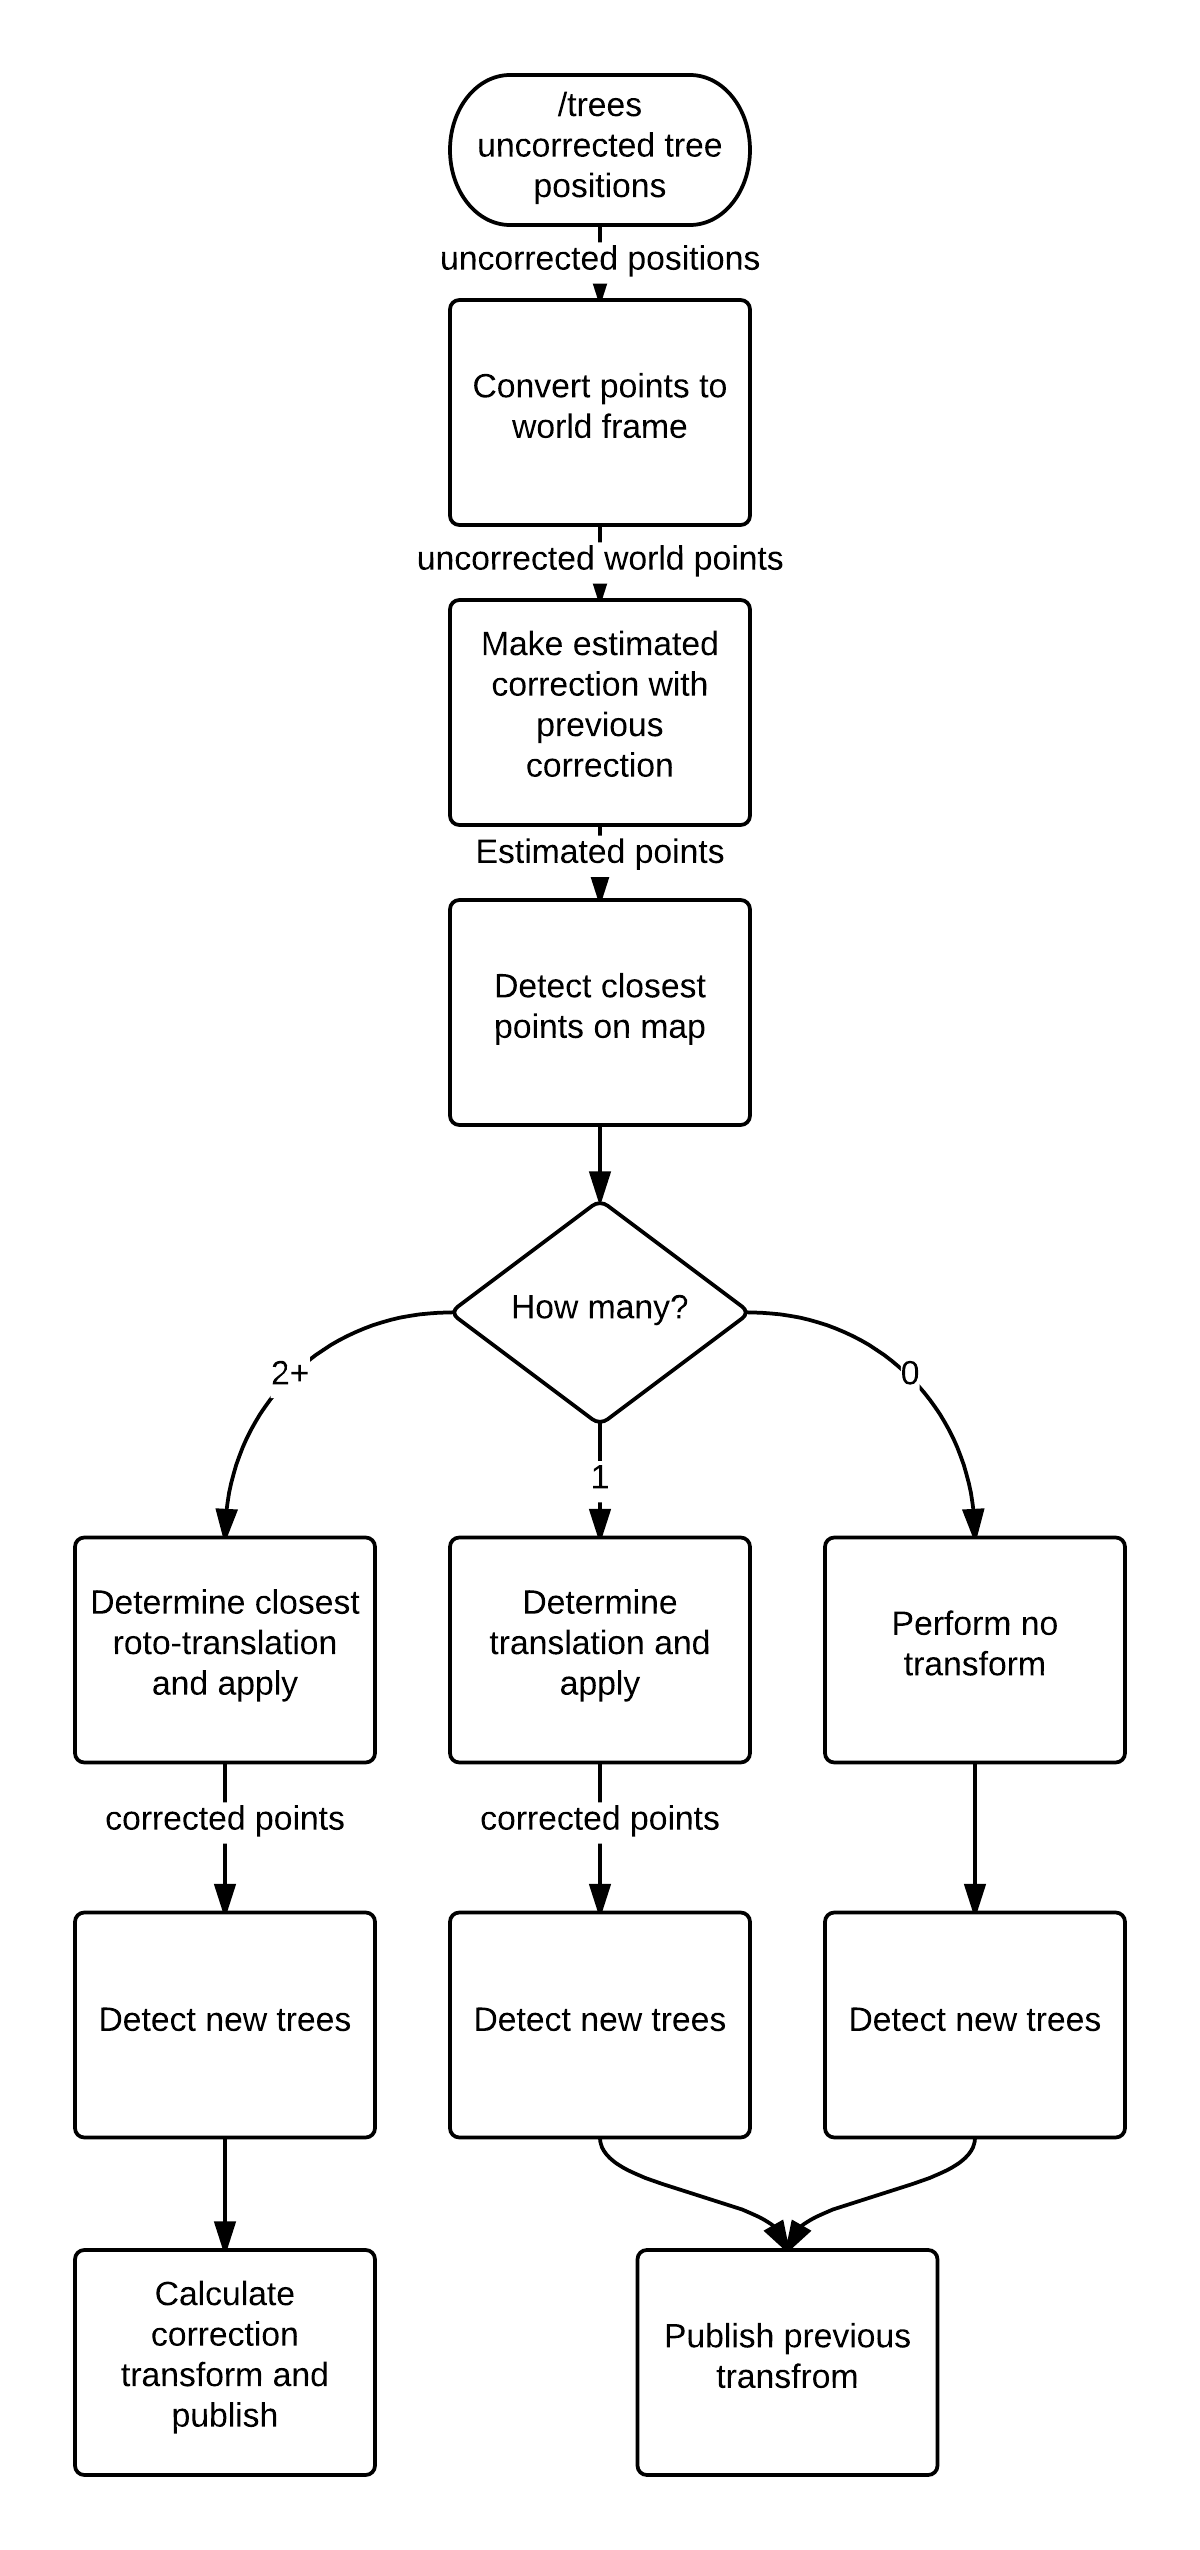
\includegraphics[width=0.65\textwidth]{figs/tree_fix}
  \caption{Flowchart describing the operation of \texttt{tree\_fix}}
  \label{fig:tree_fix}
\end{figure}

The algorithm as implemented is:
\begin{itemize}
\item Keep track of the last translation and yaw correction. Initially
  this starts at a translation of (0,0) and a yaw of 0 radians.
\item Use the last known translation and rotation to transform the
  detected points into `uncorrected points'.
\item The uncorrected points are then compared to the known
  points. Points are matched to their nearest known point, so long as
  the nearest known point is no further than a given threshold away.
\item If there are two or more points in common, a roto-translation (a
  rotation plus a translation) is then calculated such that the RMS
  error is minimised. This is done as follows. \todo{Put in proper
    equations!}
  \begin{itemize}
  \item Call the sets of points $A$ and $B$.
  \item The centroid of both set of points is taken, and subtracted
    from the every point in the set. This makes their average position
    zero. Call the new sets $A'$ and $B'$.
  \item Define a search window of $W$ radians. Try $N$ angles in
    $[-W,W]$, and for each angle construct a rotation matrix.
  \item Determine which rotation matrix minimises RMS error.
  \item Determine the translation matrix for the chosen rotation
    matrix.
  \item Return the determined matrices.
  \end{itemize}

  Previously, this was implemented using the Singular Value
  Decomposition method, but \todo{explain how it didn't work properly.}
\item If the common set only contains one point, then a simple
  translation is calculated, and it is assumed there is no rotation.
\item If there are no points in common, the transform is assumed to be
  the identity: no translation or rotation.
\item The translation is applied to all the uncorrected points, such
  that they become corrected points.
\item The corrected points are then tested against the known map
  points. If there is no map point within a given threshold distance
  of a corrected point, the corrected point is added to the map.
\item The map and the corrected points are published for visualisation
  purposes.
\item If two or more common points were detected, the correction
  converted from being in terms of the previous correction into being
  in terms of the world frame. Because the correction is prone to
  considerable jumps, it is averaged with the previous correction
  before being published. \todo{do moving average - implement and discuss}
\item If less than two points were detected, the previous correction
  is republished. It is important for smooth operation that a
  correction is published, even if it's the same - otherwise
  transforms can start to fail, leaving the system without an estimate
  of position.
\end{itemize}

Significant future work is needed on this node.  Firstly, it can be
prone to large jumps - it would be good to replace it with some form
of positioning that provides more continuous positioning. Perhaps this
could be done by integrating the position information from the polar
scan matcher and the tree matcher into a single processing node,
utilising something like a Kalman filter.

Secondly, the work on a matching algorithm seems to replicate work
done by others on scan matching. Replacing the scan matching algorithm
described with a scan matching algorithm described in the literature
should be considered. As many scan matchers are designed for laser
scans or other dense point clouds, it may be necessary to make some
changes for the vastly more sparse point cloud from the tree detector.

\section{Software Usage}
\label{sec:software-usage}

difference between realtime control and offline processing

rosbag

chunksize

\chapter{Results}
\label{cha:results}

The system can best be understood by building it up block by
block. This approach allows the performance of each major component to
be understood individually.

\section{Polar Scan Matching alone: indoor}
\label{sec:psm-indoor}

Firstly, we consider just the polar scan matcher by itself, indoors.

The polar scan matcher provides generally adequate performance inside
a room, but tends to be subject to drift and jumps. 

This is illustrated in Figure~\ref{fig:psm-indoors}, which was taken
in the RSISE building at the Australian National University. The laser
scanner started in the room in the top right corner of the scan, then
exited the room, walked straight to the corner, then turned. The
angles should be right angles, rather than the non-right angles
observed.

It's worth noting that the laser scans tend to go in `blocks':
matching will be very good for a short period (for example in a room)
then will have a `jump' where error rises significantly.

\begin{figure}[h!]
  \centering
  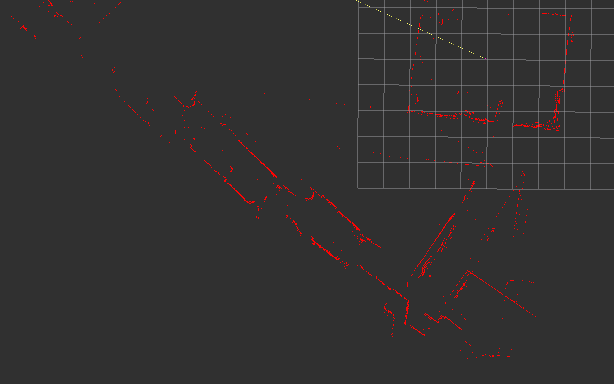
\includegraphics[width=\textwidth]{figs/indoor}
  \caption{Performance of polar scan matcher alone, indoors.}
  \label{fig:psm-indoors}
\end{figure}

A few observations can be made about the jumps:
\begin{itemize}
\item Part of the reason was traced back to sensor/recording
  error. \texttt{rosbag}, which was used to record the data, saves the
  data out in chunks of a certain size. By default, the chunk size is
  768 KB. Unfortunately, writing that much data out to the CF card
  used in the onboard computer caused noticeable delay. This was
  reduced later in development to 256 KB, which reduced the delay.
\item Performance in corridors was particularly bad. This was at least
  partially due to the self-similarity of corridors: without either
  being able to see the end of a corridor or other distinguishing
  landmarks, and with no IMU or other form of odometry, it becomes
  difficult to distinguish movement from staying stationary.
\item Turning corners and leaving rooms seemed to be particularly
  large sources of error. This could be due to the particularly large
  number of points changing quickly, with very few points remaining
  across the turn.
\end{itemize}

It was also interesting to note that if one of the SLAM systems that
is available with ROS was added to the system (for example
\texttt{slam\_gmapping}), performance improved significantly
indoors. However, the chunking issue identified above still tended to
cause problems.

As indoor navigation was not a priority, merely an early way to test
the system, no major work was invested in ironing out defects. Rather,
the system was tested outdoors.

\section{Polar Scan Matching alone: outdoor}
\label{sec:psm-outdoor}

The polar scan matcher was then tested outdoors.

Initially, the system was entirely unusable, not detecting motion in
any usable way whatsoever. Firstly, a greater range laser scanner
was tried, as explained in Section~\todo{ref}. However, ultimately
various fixes to the software were required. These are explained in
Section~\ref{sec:polar-scan-matcher}.

Once those fixes were deployed, the polar scan matcher provided
estimates which were roughly correct, especially in the short term,
but which tended to drift unacceptably. The drift was especially
visible on tree trunks, which became ``blurred'', as shown below in
Figure~\ref{fig:blur-detailed}. 

\begin{figure}[h!]
  \centering
  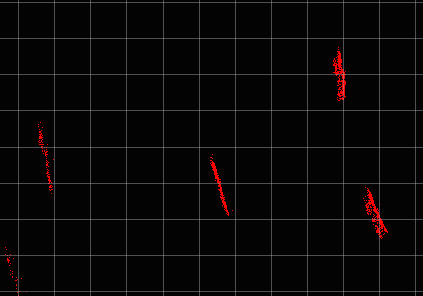
\includegraphics[width=0.8\textwidth]{figs/blurring}
  \caption{``Blurring'' experienced by uncorrected outdoor polar scan matching.}
  \label{fig:blur-detailed}
\end{figure}

The cumulative drift and error is
significant. Figure~\ref{fig:psm-outdoor} shows the result of walking
the scanner assembly around a clump of trees at ANU \todo{ref to the
  particular clump}. The path taken was a loop - the net translation
should be zero. However, a large translation is observed; trees do not
stay in the same place and there is lots of noise.

\begin{figure}[h!]
  \centering
  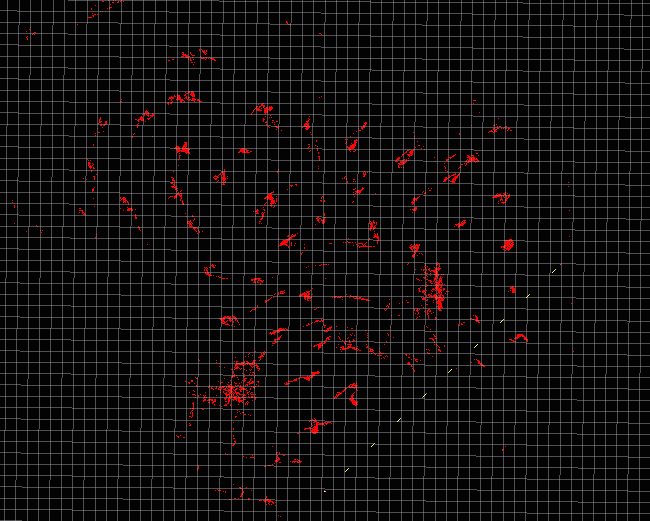
\includegraphics[width=0.9\textwidth]{figs/psm-outdoor}
  \caption{PSM only, outdoors}
  \label{fig:psm-outdoor}
\end{figure}

Evidently further work was required for accurate localisation.

\section{Tree-based localization}
\label{sec:tree-based-local}

Adding the tree-based localization described in
Section~\ref{sec:tree-detection-localization} led to significant
improvement in results. Two major outdoor locations were tested.

\subsection{Tennis Court}
\label{sec:tennis-court}

The ``tennis court'' location is a clump of trees near some tennis
courts on the ANU campus. The trees are pictured in
Figure~\ref{fig:tennis-trees}.

\begin{figure}
  \centering
  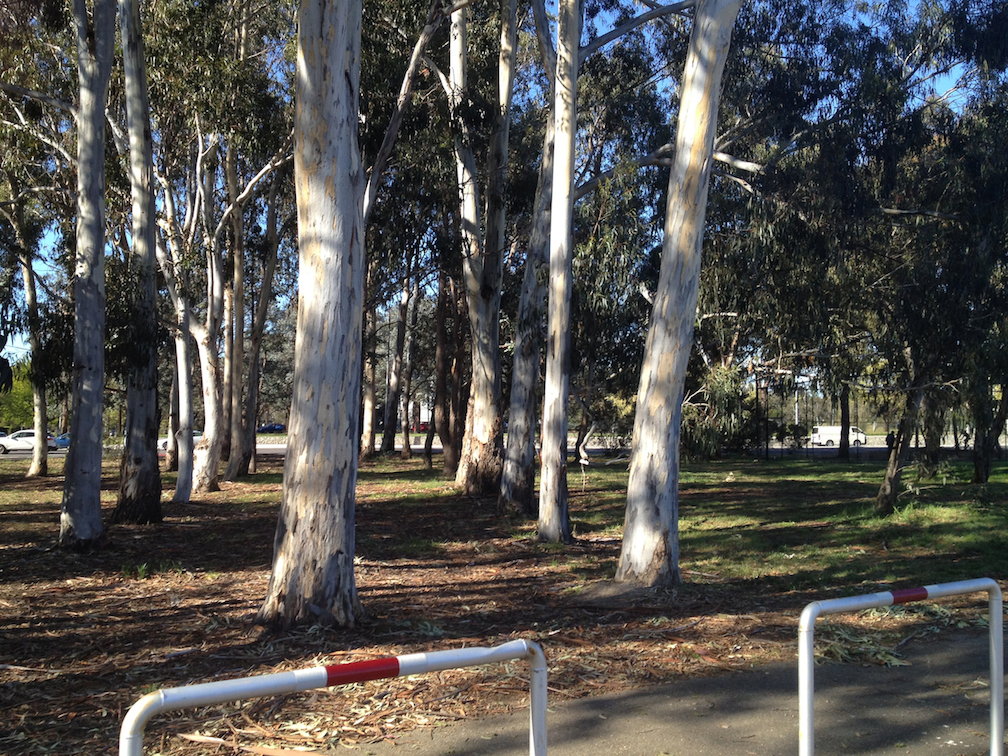
\includegraphics[width=0.6\textwidth]{figs/tennis-1}\\
  ~\\
  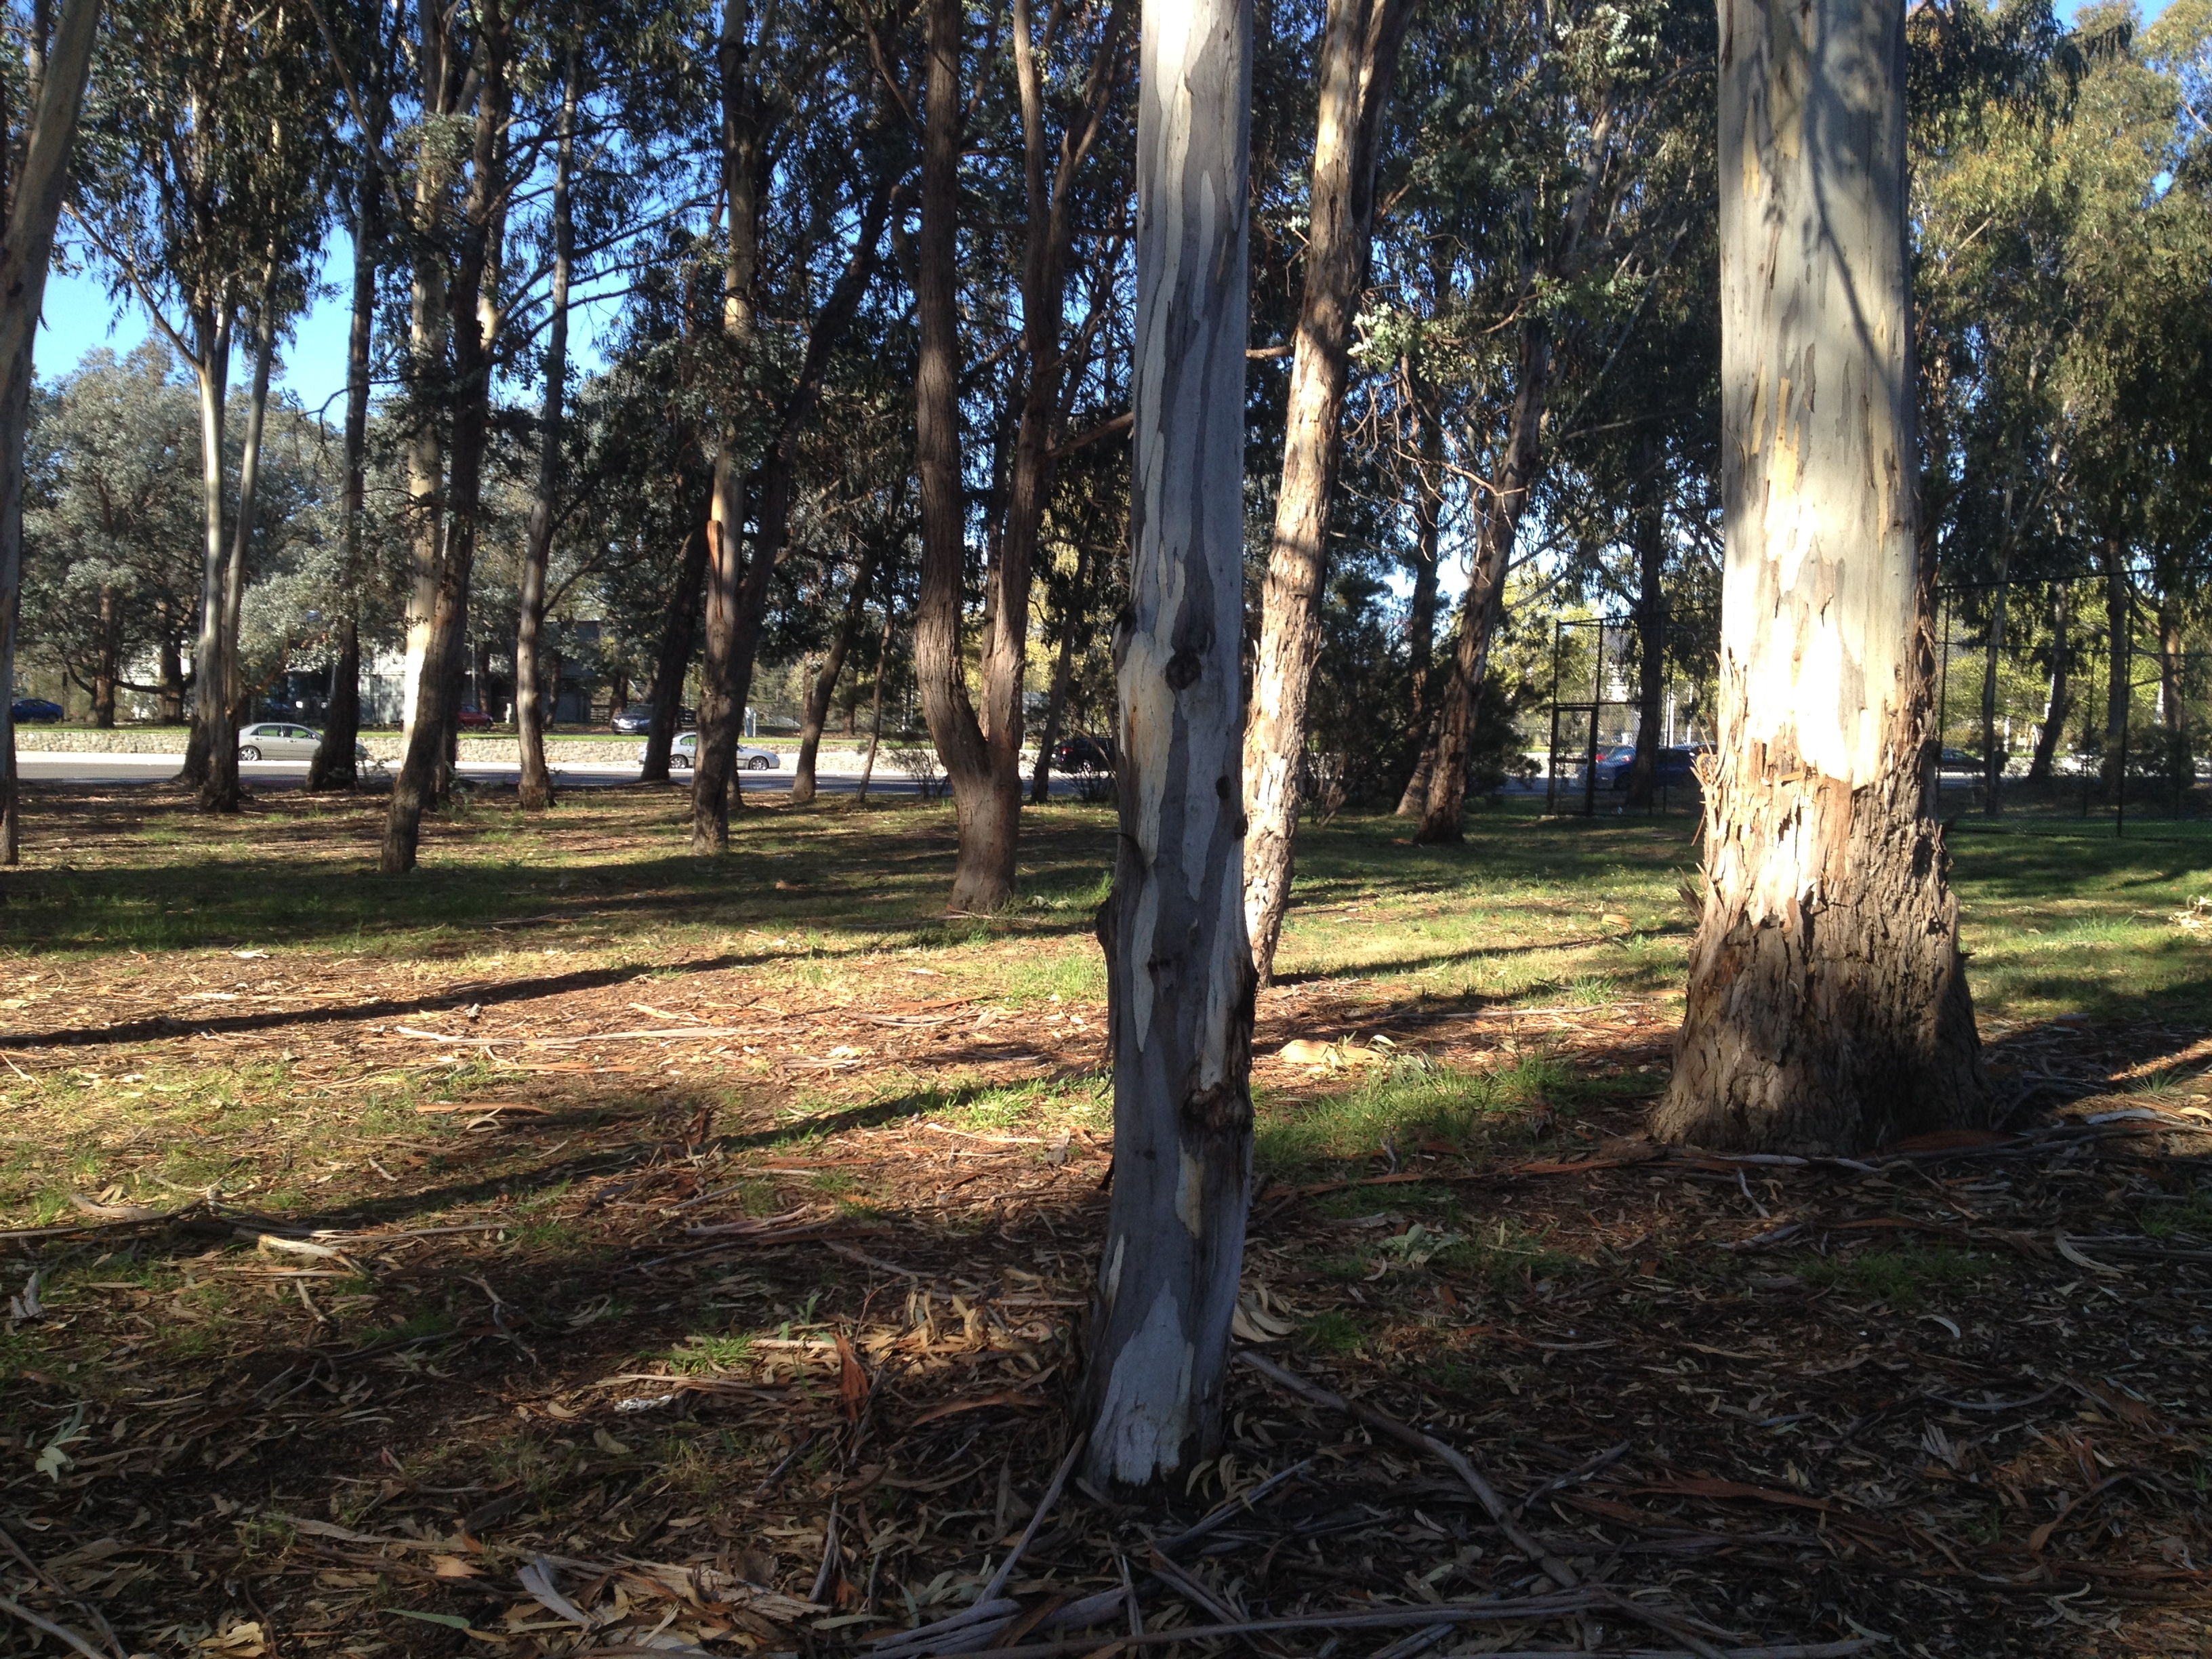
\includegraphics[width=0.6\textwidth]{figs/tennis-2}\\
  ~\\
  \includegraphics[width=0.6\textwidth]{figs/tennis-3}\\
  \caption{Various pictures of the ``tennis court'' clump of trees.\\
  \textbf{Top:} View from the start of the loop (the dented metal
  rail).\\
  \textbf{Middle:} View from mid-way though the loop.\\
  \textbf{Bottom:} View from towards the end of the loop.}
  \label{fig:tennis-trees}
\end{figure}

The hexacopter landing gear assembly was walked in a loop through the
clump of trees.

The results: the path taken and the map of trees detected is shown in
Figure~\ref{fig:tennis-results}. \todo{Video and data bag location}

\begin{figure}
  \centering
  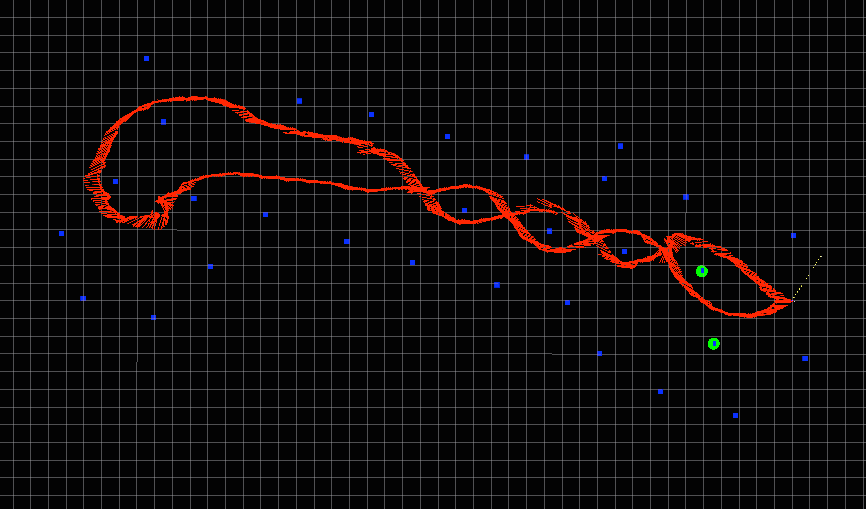
\includegraphics[width=0.9\textwidth]{figs/tennis-results}\\
  ~\\
  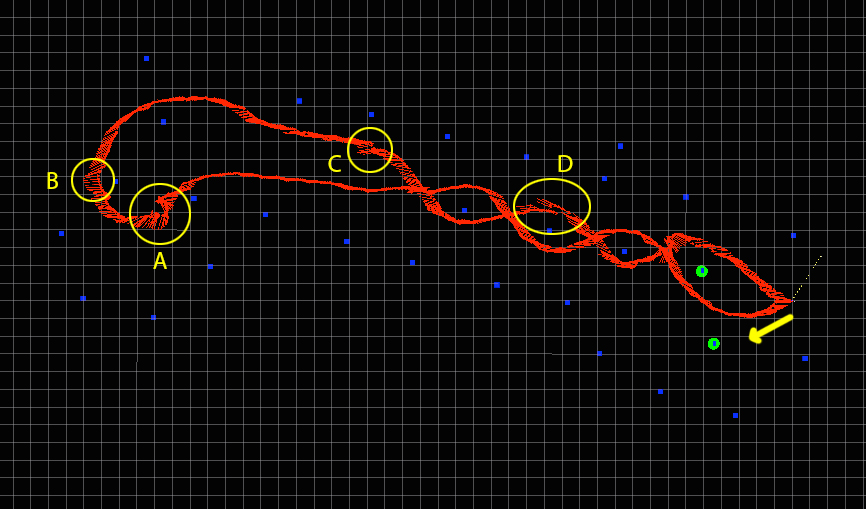
\includegraphics[width=0.9\textwidth]{figs/tennis-results-annotated}
  \caption{Tennis Results. \textbf{Top:} raw results. \textbf{Bottom:}
  annotated results.}
  \label{fig:tennis-results}
\end{figure}

The landing gear was walked in a loop. Initially, the 

While walking, \begin{itemize}
\item Keep in view of multiple trees
\item Discontinuous/not always available; jumps
\end{itemize}

In the results:
\begin{itemize}
\item The \emph{red line} represents the path travelled. The line is a
  collection of arrows, where the base of each arrow represents the
  position at that instant, and the arrow is facing in the direction
  the landing gear was facing.
\item The \emph{green dots} represent trees \emph{currently being
    detected} by the tree detection algorithm. In this case, two trees
  in view of the start/end position are detected.
\item The \emph{blue dots} represent the position of every tree known
  to the system, the `map'.
\end{itemize}

The results have been annotated to highlight several
features. Firstly, the arrow shows the initial direction of movement
along the loop. The labelled regions are as follows:
\begin{enumerate}[A:]
\item This region shows the landing gear being rotated around a
  point. This was done to ensure that the scanner remained in view of
  multiple trees for as much of the route as possible.
\item This region shows the landing gear being walked sideways: unlike
  early in the path, the arrows are perpendicular to the direction of
  travel. Again this was done to ensure that the laser scanner had a
  good view of trees.
\item This shows a simple `jump' in position, as the system goes from
  being able to see one tree, and therefore not being able to do a
  position correction, to seeing two trees, and being able to do a
  position correction. The averaging algorithm reduces the level of
  discontinuity in the position, but the discontinuity is still
  observable.
\item This shows a more complicated `jump', as the system became
  momentarily confused about its position, and then recovered.
\end{enumerate}

Because the path was a loop, we can consider how accurately the path
closes. Over a distance of around 40m each way, the final position was
virtually indistinguishable from the original position\todo{, with error of
around 10cm. double check}

As such, we can conclude that the algorithm was highly successful for
this set of trees.

\subsection{Roadside}
\label{sec:roadside}

The ``roadside'' location is another clump of trees on the ANU
campus. The trees are pictured in Figure~\ref{fig:roadside-trees}.

\begin{figure}
  \centering
  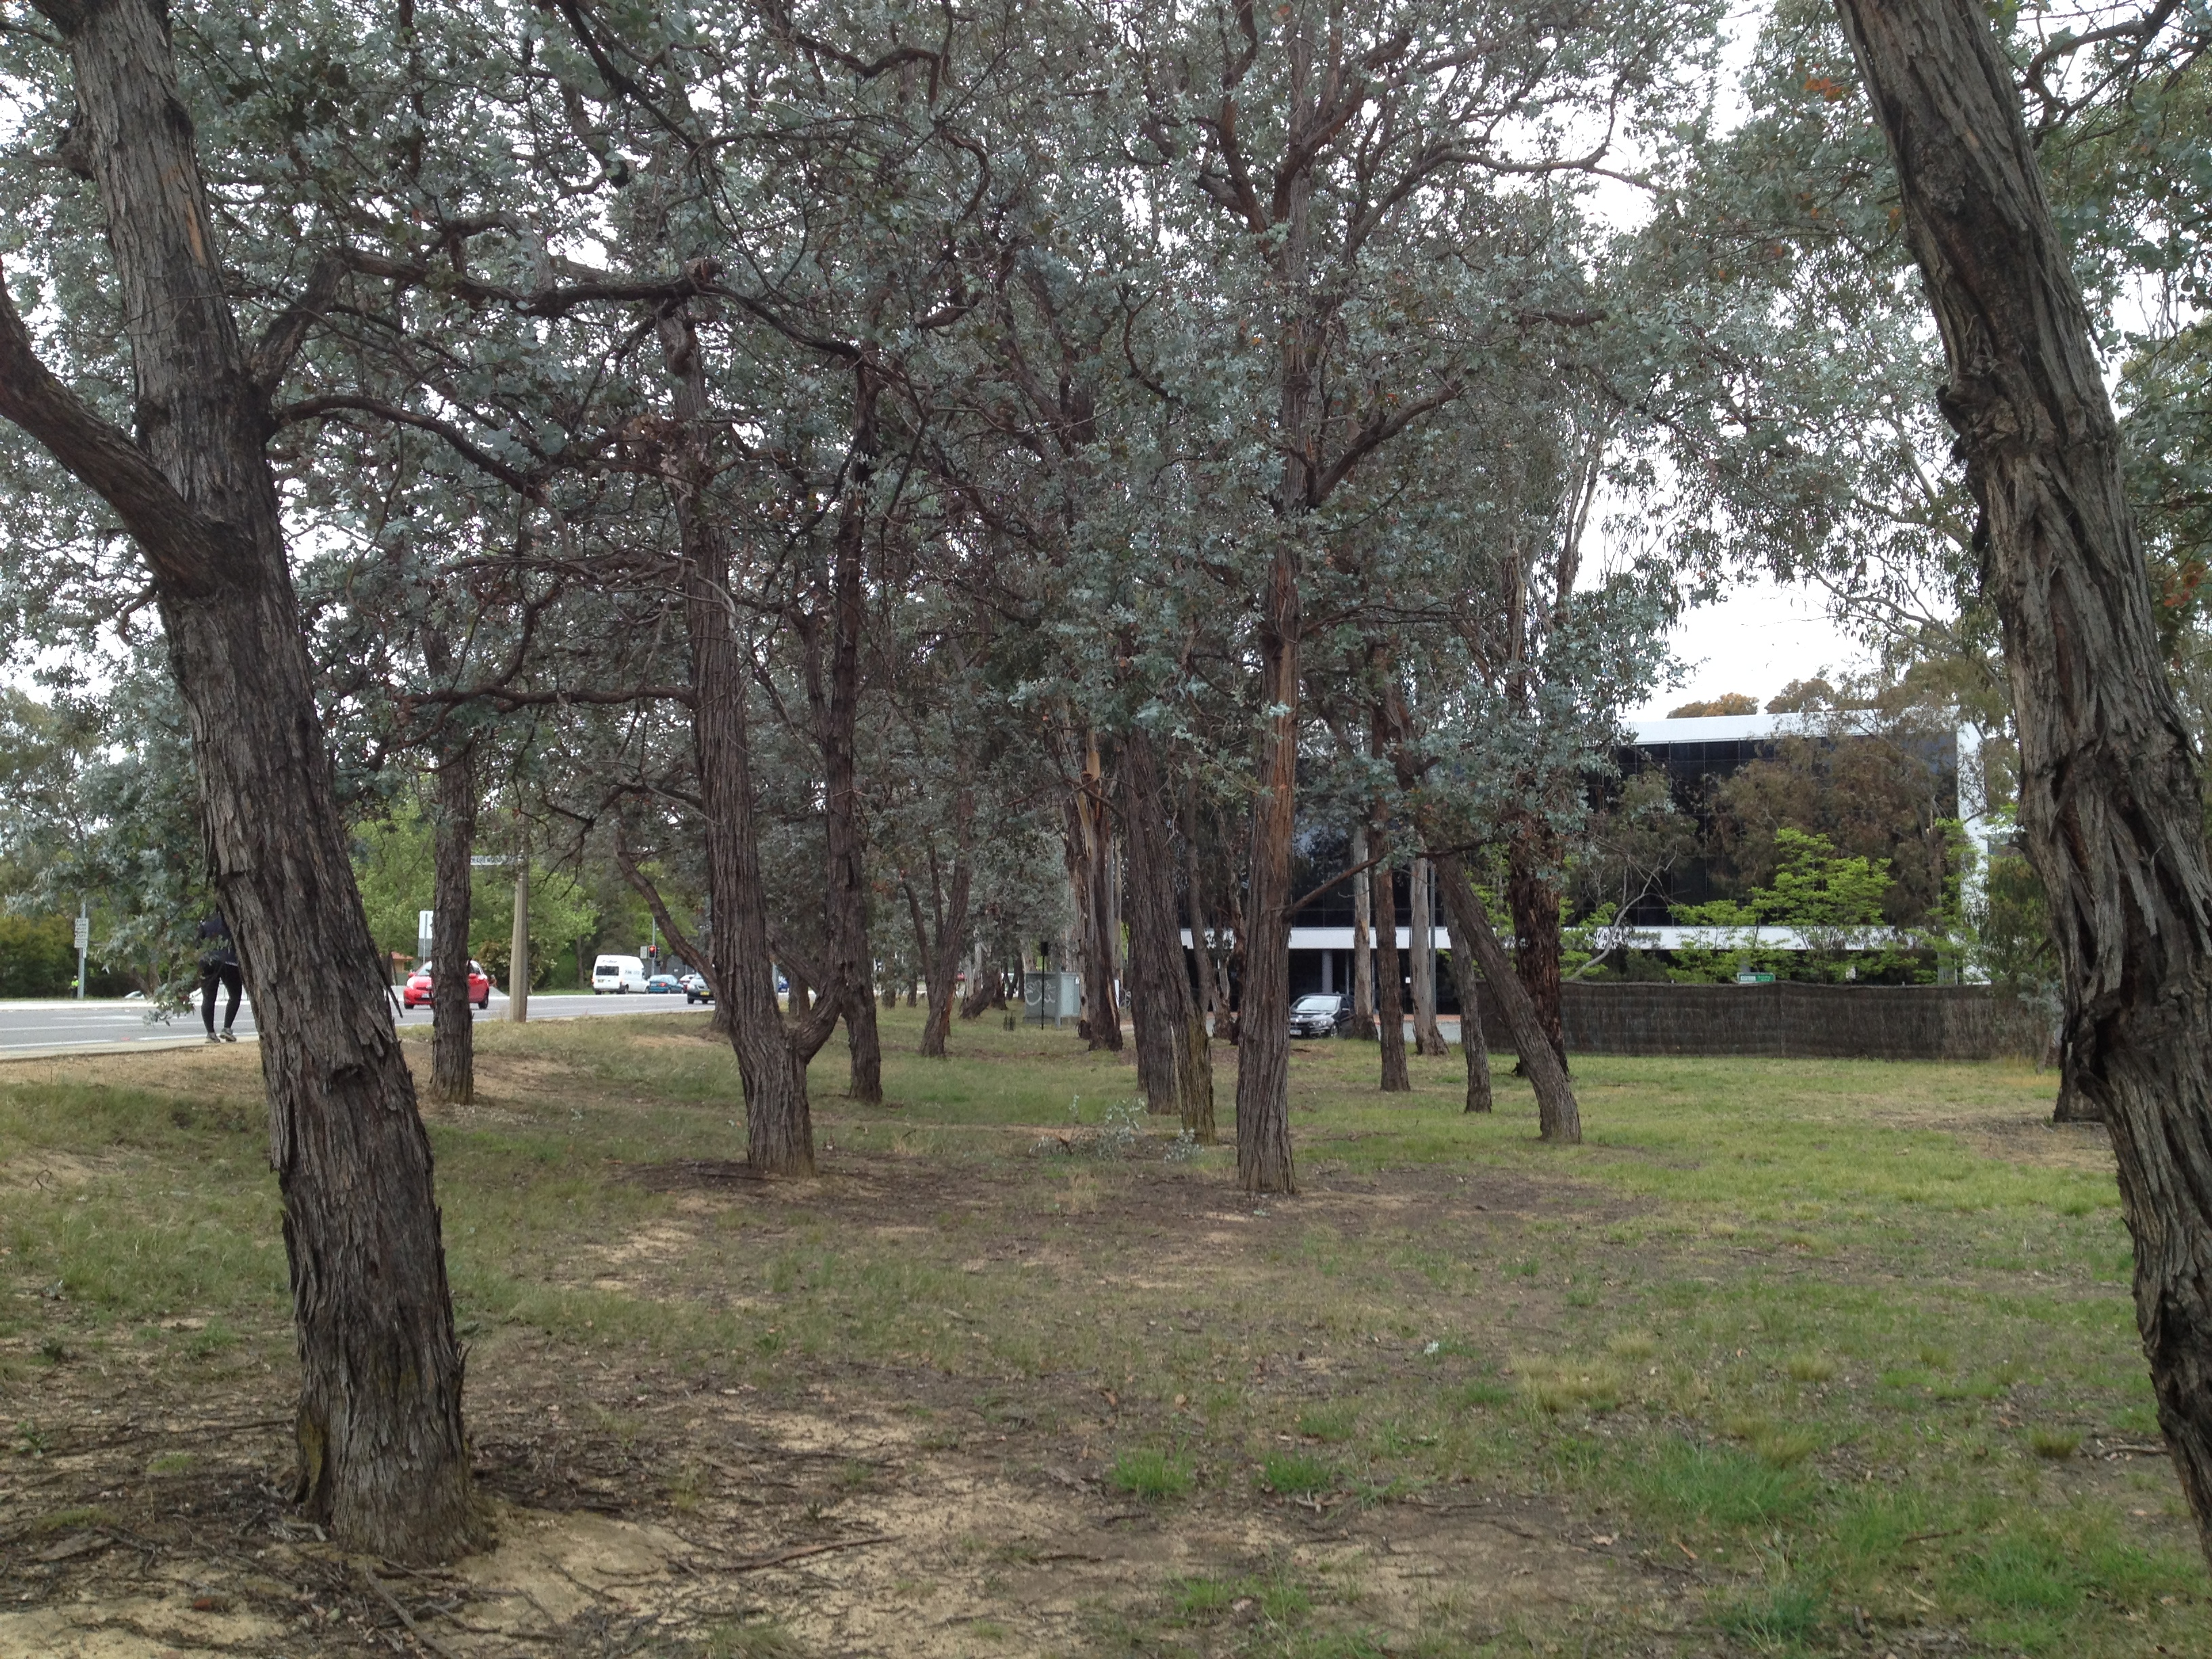
\includegraphics[width=0.8\textwidth]{figs/roadside-1}
  \caption{Roadside trees}
  \label{fig:roadside-trees}
\end{figure}

Again the hexacopter landing assembly was walked in a loop, with the
results plotted in Figure~\ref{fig:roadside-results}.

\begin{figure}
  \centering
  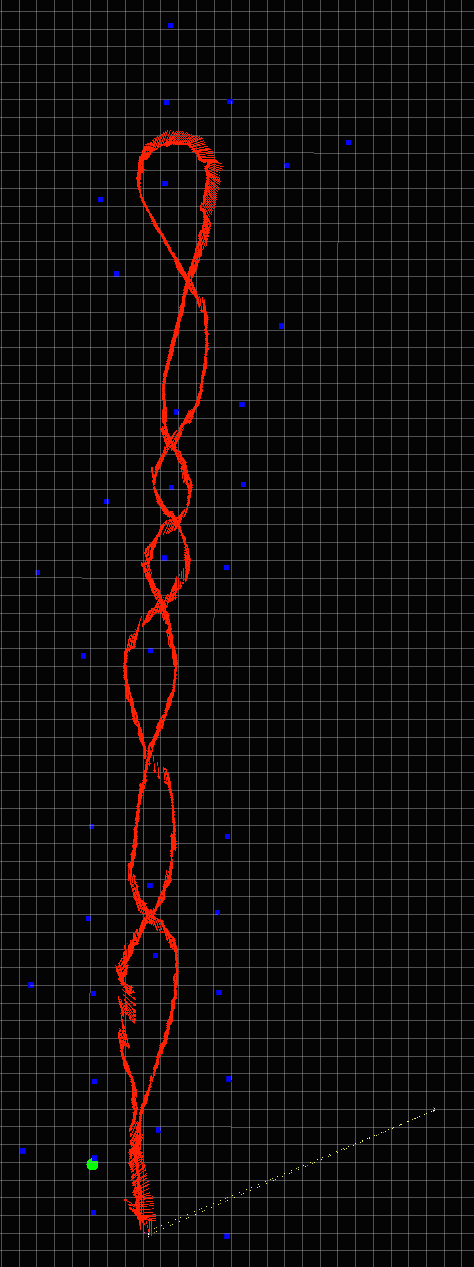
\includegraphics[width=0.45\textwidth]{figs/roadside-results}
  ~
  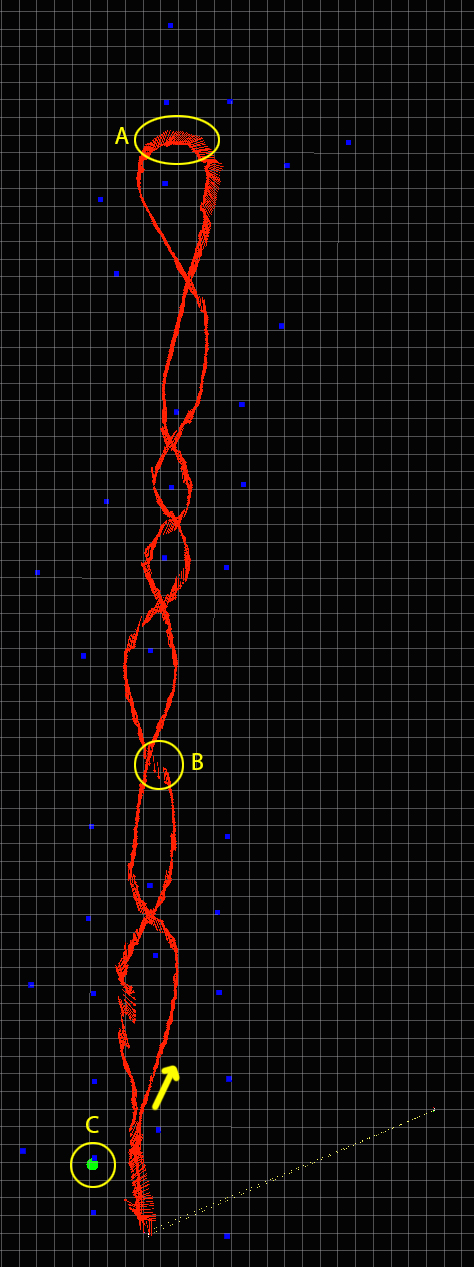
\includegraphics[width=0.45\textwidth]{figs/roadside-results-annotated}
  \caption{Roadside results. \textbf{Left:} unannotated
    results. \textbf{Right:} annotated results}
  \label{fig:roadside-results}
\end{figure}

The symbols are the same as in the previous location.

Points to note include:
\begin{enumerate}[A:]
\item The landing gear was again walked perpendicular to the direction
  it was facing at the end of the loop in order to get a clear
  reading.
\item There were a number of significant jumps. This jump has been
  highlighted because it occurs after a reasonably large chunk of
  having no trees detected at all (note the large `gap' in trees
  directly above it on the map), so it provides a good example of
  the amount of small-scale drift experienced over moderate distances
  when using PSM alone.
\item Unlike the previous example, this example does not end with two
  trees visible, but only one. As shown here, the detected tree starts
  to drift off from the known tree, because corrections can only be
  correctly estimated with two trees. This demonstrates that PSM
  drifts away from the ground truth even in the absence of motion.
\end{enumerate}

The return to origin behaviour is excellent when in view of two trees,
but does, as this example shows, tend to drift away when only one tree
is in view. However, once that is accounted for, the accuracy is very
good --- this time over a distance of about 60 meters each way.

\subsection{Negative results}
\label{sec:negative-results}

Along with the two successful results above, there were a number of
unsuccessful trials. While all the trials were different, a number of
observations can be made, which further characterise the system.

There are two major reasons for unsuccessful trials: sensor and
recording errors, and algorithm errors. Recording errors will be
detailed here, and algorithm errors discussed in \todo{ref:discussion
  of negative results}

There were two major sources of recording error. Firstly, the chunking
error discussed in Section~\ref{psm-indoor}. Secondly, there were some
issues with the recorded data missing the start and/or end of the
route. This was mitigated by using a smaller chunk size, and
ultimately eliminated by waiting 10--15 seconds from when the system
started.

\subsection{Conclusion --- walking only}
\label{sec:concl-walk-only}

The results from walking the landing gear around the two locations are
highly positive.

In short, they demonstrate that:
\begin{itemize}
\item  the hardware works and is capable of
handling the low-frequency vibrations and general `wobble' caused by
being walked around.
\item the software works, both in terms of being able to record and
  replay data, and also in the sense of being able to successfully
  localise the platform as it is being walked around.
\item the software works in both locations, so it is not overly
  specialised for a single location or set of assumptions.
\end{itemize}

However, just walking around leaves a few questions: can the hardware
handle flying, especially in terms of high frequency vibrations; and
can the software handle the extra `noise' in the data caused by flying?

\section{Flying}
\label{sec:flying}

The landing gear was attached to one of ANU's hexacopters. The
hexacopter power was kept separate from the landing gear power, in
order to prevent any drops in voltage from sudden acceleration from
causing issues with the computer.

The hexacopter was able to take off, but required around 70\%
throttle, suggesting the overall weight should be reduced.

Two flight tests were undertaken, which are explored below.

\subsection{RSISE}
\label{sec:rsise}

The first flight test was conducted outside the Research School of
Information Sciences and Engineering at ANU. The clump of trees used
is shown in Figure~\ref{fig:rsise-trees}. The hexacopter in flight is
shown in Figure~\ref{fig:rsise-flying}.

\begin{figure}
  \centering
  \includegraphics[width=0.9\textwidth]{figs/rsise-trees-1}\\
  ~\\
  \includegraphics[width=0.9\textwidth]{figs/rsise-trees-2}
  \caption{RSISE Trees\\\textbf{Top:} View showing the front/side
    showing the big tree, 2 front trees
    and the 2 back trees.\\\textbf{Bottom:} View from the side, looking
  in the opposite direction.}
  \label{fig:rsise-trees}
\end{figure}

\begin{figure}
  \centering
  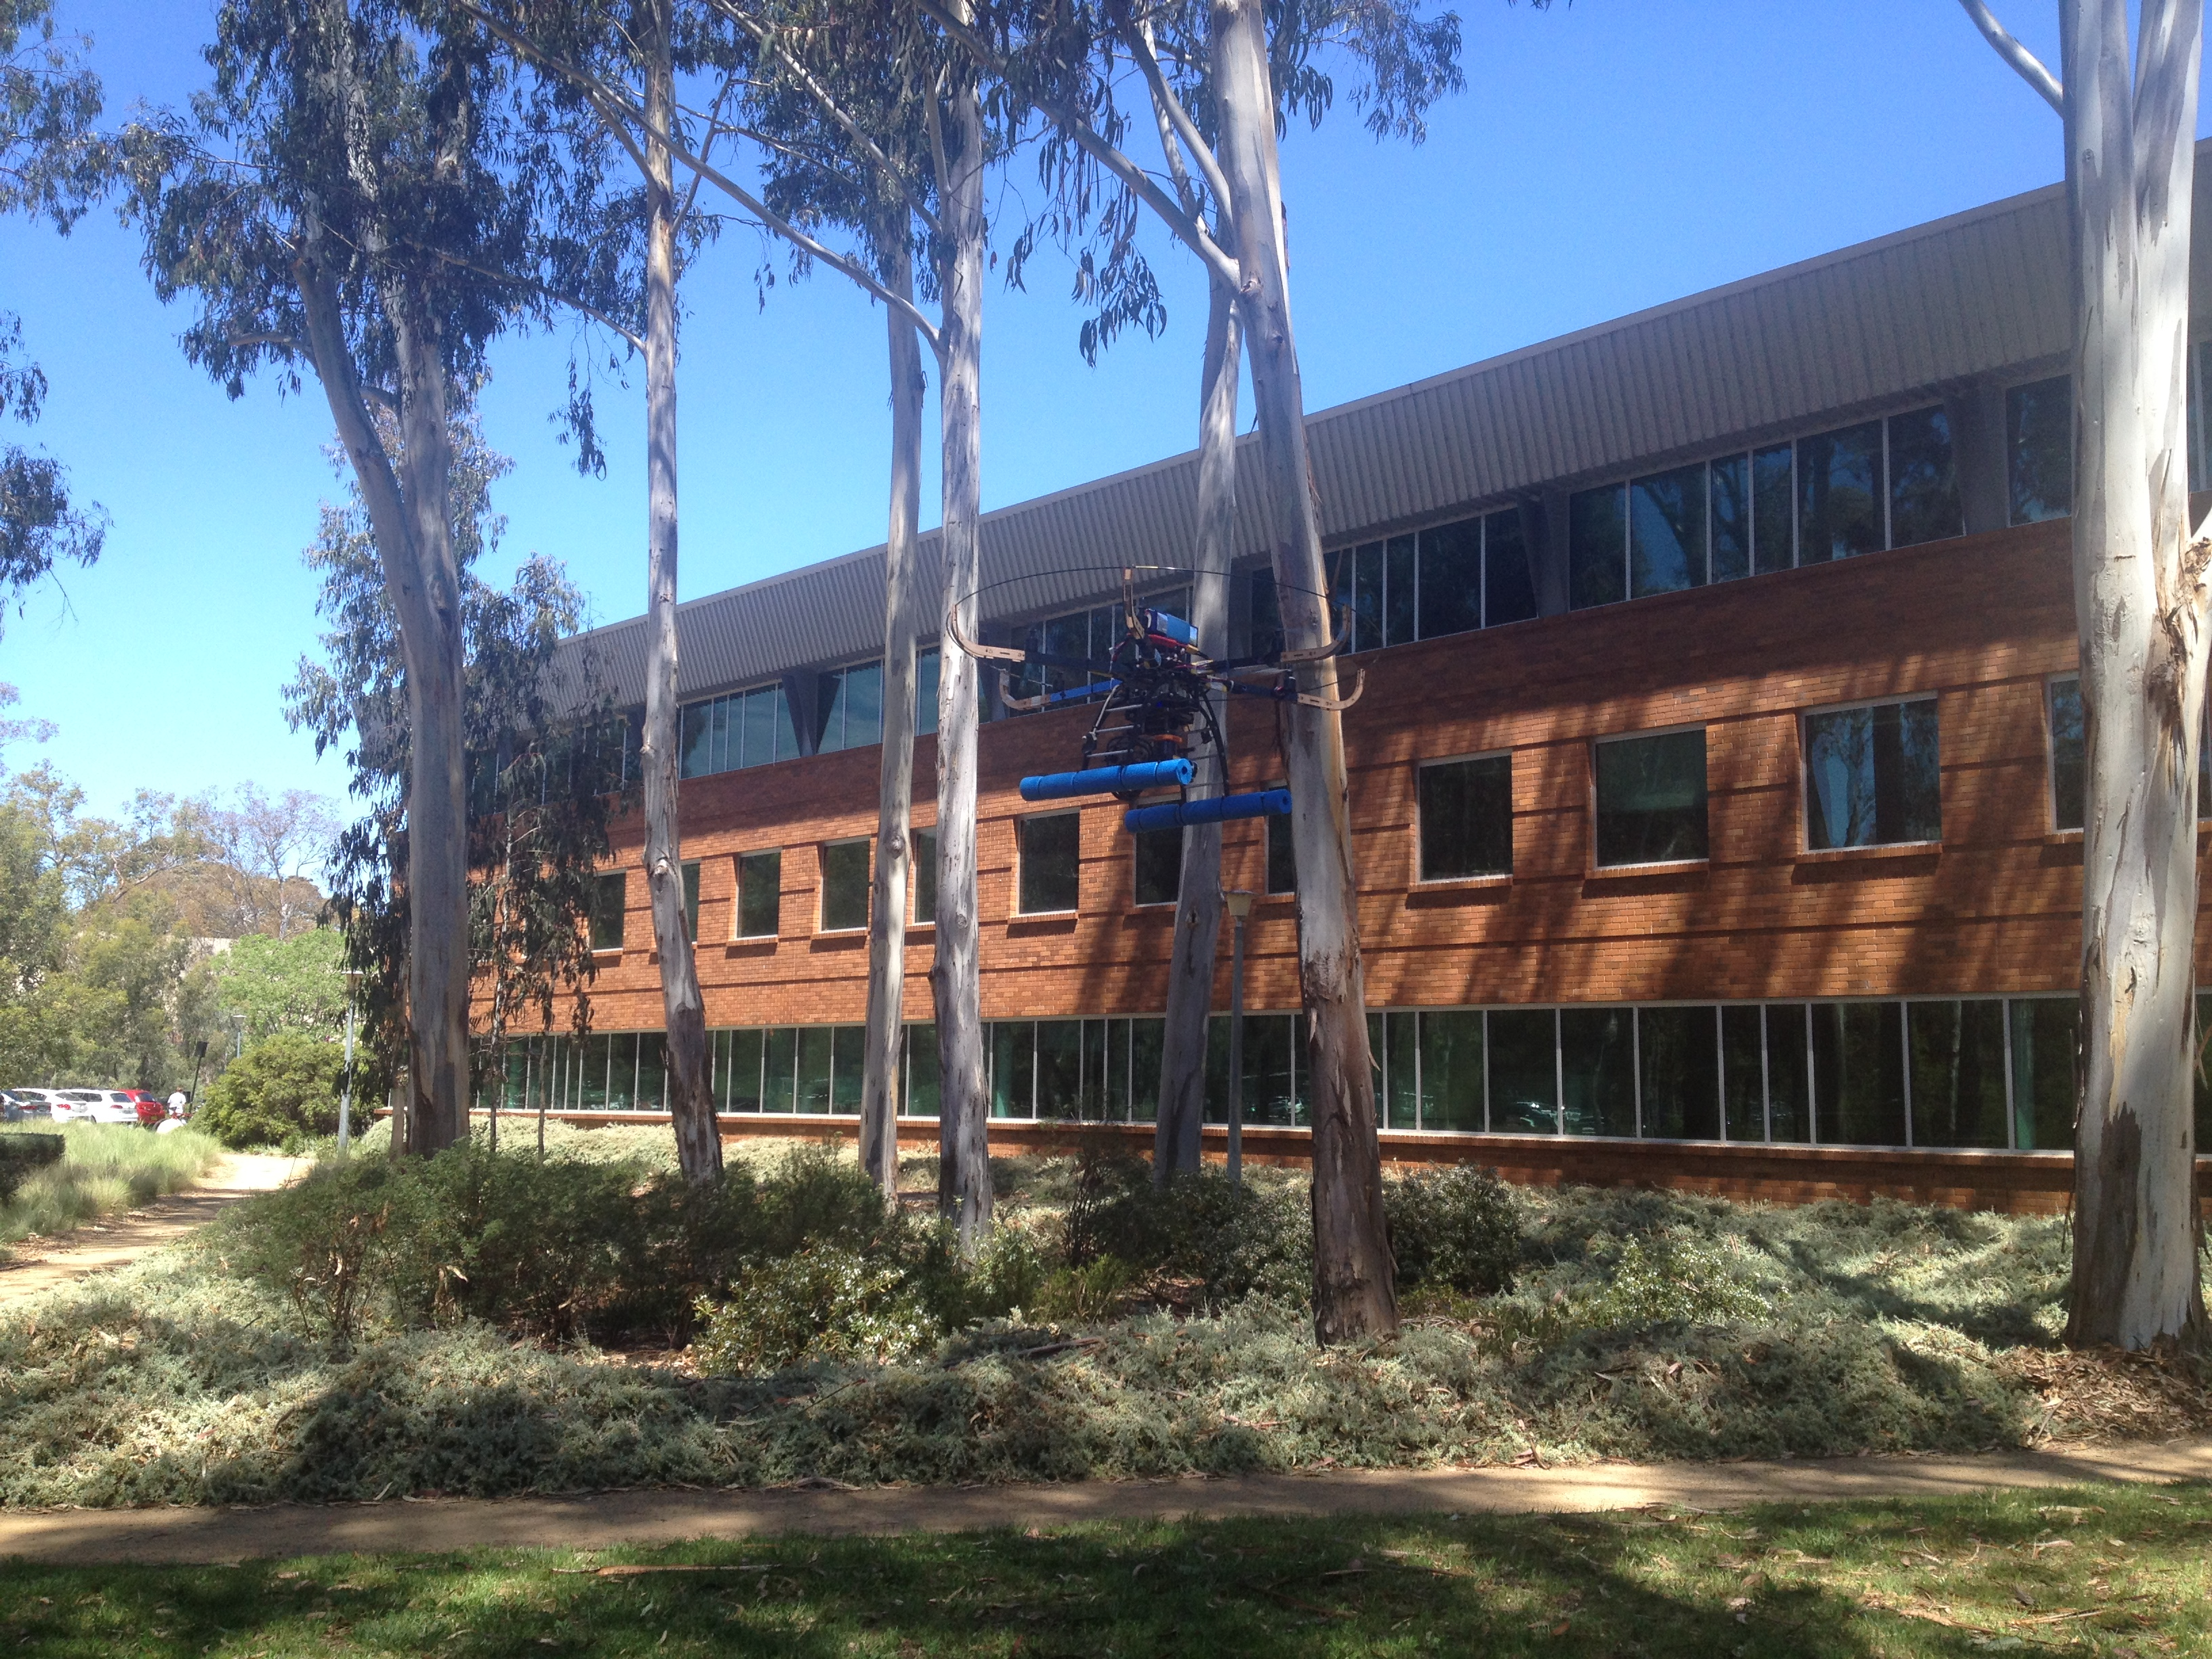
\includegraphics[width=0.9\textwidth]{figs/rsise-flying}
  \caption{The hexacopter flying near the RSISE trees}
  \label{fig:rsise-flying}
\end{figure}

\subsection{Tennis Court}
\label{sec:tennis-court-1}



\chapter{Discussion}
\label{cha:discussion}

Discussion of negative results while walking:
 - The system is very sensitive to the PSM. Sudden jumps, greater than
 the thresholds, will just cause everything to go to hell. On the
 other hand we don't want to change that threshold too much because it
 will cause a jump-back e.g. in the roadtrees B.
 - PSM is pretty bad at dealing with circling a single tree. This
 makes sense: a circle from any angle looks the same, so it's not
 surprising.
 - Likewise PSM just epically fails if things are sparse; hence RSISE
 worse than all.

\chapter{Conclusion}
\label{cha:conclusion}


%%%%%%%%%%%%%%%%%%%%%%%%%%%%%%%%%%%%%%%%%%%%%%%%%%%%%%%%%%%%%%%%%%%%%%
% Here begins the end matter

%\input appendix

\backmatter
\bibliographystyle{IEEEtran}
\bibliography{IEEEabrv,report}

\end{document}

%%% Local Variables: 
%%% mode: latex
%%% TeX-master: "report"
%%% End: 



